%%
%% This is file `thesis.tex',
%% generated with the docstrip utility.
%%
%% The original source files were:
%%
%% scnuthesis.dtx  (with options: `thesis')
%% 
%% !Mode:: "TeX:UTF-8"
%% 
%% This is a generated file.
%% 
%% Copyright (C) 2013 by Joseph Pan <cs.wzpan@gmail.com>
%% 
%% This file may be distributed and/or modified under the
%% conditions of the LaTeX Project Public License, either version 1.3a
%% of this license or (at your option) any later version.
%% The latest version of this license is in:
%% 
%% http://www.latex-project.org/lppl.txt
%% 
%% and version 1.3a or later is part of all distributions of LaTeX
%% version 2004/10/01 or later.
%% 
%% To produce the documentation run the original source files ending with `.dtx'
%% through LaTeX.
%% 
%% Any Suggestions : Joseph Pan <cs.wzpan@gmail.com>
%% Thanks LiuBenYuan <liubenyuan@gmail.com> for the nudtpapre class!
%% Thanks Xue Ruini <xueruini@gmail.com> for the thuthesis class!
%% Thanks sofoot for the original NUDT paper class!
%% 
%1. 如果是研究生论文,常用的选项是:
% \documentclass[master,twoside,vista,ttf]{scnuthesis}
%2. 如果是博士生论文,常用的选项是:
% \documentclass[doctor,twoside,vista,ttf]{scnuthesis}
%3. 如果使用是Windows XP之前的Windows系列,或者使用从这个系列拷贝过来的字体,则需要将Vista选项去掉,如:
% \documentclass[master,twoside,ttf]{scnuthesis}
%4. 建议使用OTF字体获得较好的页面显示效果
%   OTF字体从网上获得,各个系统名称统一,不用加vista选项
%   如果你下载的是最新的(1201)OTF英文字体,建议修改scnuthesis.cls,使用PS Std
%   \documentclass[doctor,twoside,otf]{scnuthesis}
%5. 如果想生成盲评,传递anon即可,仍需修改个人成果部分
% \documentclass[master,otf,anon]{scnuthesis}
%6. 让章节标题作为页眉,可以使用chapterhead选项。如果和twoside一起使用,则奇数页页眉为章节标题,偶数页为文章标题。
% \documentclass[master,otf,twoside,chapterhead]{scnuthesis}
%
\documentclass[master,otf,twoside]{scnuthesis}
\usepackage{myscnu}

\begin{document}
\graphicspath{{figures/}}
\classification{}
\university{10574}
\confidentiality{无}
\serialno{2011022078}
%\title{基于前景跟踪和多尺度混合的\\欧拉影像放大技术}
%\entitle{EULERIAN VIDEO MAGNIFICATION BASED ON FOREGROUND-TRACKING AND MULTI-RESOLUTION BLENDING}
\title{前景约束的欧拉影像动作放大技术}
\entitle{FOREGROUND-CONSTRAINED EULERIAN VIDEO MOTION MAGNIFICATION}
\displaytitle{前景约束的欧拉影像动作放大技术}
\author{潘伟洲}
\enauthor{Weizhou Pan}
\subject{计算机应用技术}
\ensubject{Computer Applications Technology}
\researchfield{数字图像处理}
\school{计算机学院}
\supervisor{李兴民}
\ensupervisor{Xingmin Li}
\protitle{教授}
\zhdate{\zhtoday}
% 插入摘要,制作封面
\ifisanon{}\else{\maketitle}\fi
\frontmatter
\begin{cabstract}
  影像动作放大技术是一种用于改变影像中感兴趣信号的变化幅度的技术。这类技术可以将
  生活中原本裸眼无法感知的微弱变化放大到裸眼可以感知的幅度,从而挖掘出有价值的信
  息。

  根据视角的不同,影像动作放大技术分为拉格朗日视角和欧拉视角两种视角。其中,拉格
  朗日视角的方法通过跟踪和改变粒子的运动轨迹来放大变化,但容易受到遮挡的影响,且
  需要在后期对背景进行填充;欧拉视角的方法则通过分析和增强图像的像素点的灰度值随
  时间的变化来放大变化,但对于已存在大幅度变化的场景,使用该方法会造成明显的“鬼
  影”现象。

  本文提出了一种结合了拉格朗日视角和欧拉视角的优点的影像动作放大方法,该方法在欧
  拉影像动作放大技术的基础上,通过使用目标跟踪技术,将放大区域限制在由用户选定的
  感兴趣区域上。同时,通过使用前景分割技术,将经过放大的动作与感兴趣区域的前景部
  分进行多分辨率混合。

  实验结果表明,该方法应用在已存在大幅度变化的场景时可以有效
  的避免“鬼影”问题。此外,将放大的区域限制在感兴趣的区域,可以减少场景中的其他
  部分对该区域的干扰,有利于对放大结果的后续分析。
  
\end{cabstract}
\ckeywords{欧拉影像放大技术;目标跟踪;Mean-shift;GrabCut;多分辨率混合}

\begin{eabstract}
  Video motion magnification is a kind of techniques for changing the motion
  amplitude of signal of interest from videos. With such techniques we are able
  to reveal subtle changes in the world that are originally invisible to naked
  eyes, so as to exploit valuable information.

  Video motion magnification techniques follow two different perspectives
  \textsl{i.e.} Lagrangian perspective or Eulerian perspective. On one hand,
  methods following Lagrangian perspective amplify motions by tracking and
  modifying the trajectory of particles, but it is easy to introduce artifacts
  especially at region of occlusion boundaries and may require image-inpainting
  as post-processing. On the other hand, methods following Eulerian perspective
  amplify motions by analyzing and enhancing the variation of pixel values that
  evolve over time. However, if the input video contains large motions, the
  magnified video will suffer from artifacts that known as ghosting effect.

  This paper presents a method that takes the advantages of both two
  perspectives. Based on eulerian video magnification, we perform object
  tracking to constrain the amplifying area to a region of interest that is
  selected by the user. At the same time, our method relies on a foreground
  segmentation for multi-resolution blending the amplified motion with the
  foreground part of the original region.

  The experimental results show that the
  approach can obviously eliminate ghosting effect when processing videos with
  large motions. Besides, by constraining the amplifying area to a region of
  interest, it can significantly reduce interference from other parts of the
  scene, which is beneficial to further studies on the amplified results.
\end{eabstract}
\ekeywords{eulerian video magnification; object tracking; Mean-shift; GrabCut;
  multi-resolution blending}

% 生成目录
\tableofcontents
% \listoftables           % 如果要生成表目录
% \listoffigures          % 如果要生成图目录

\renewcommand{\chapterlabel}{\denotationname} %设置页眉

% \begin{denotation}

\item[SCNU] 华南师范大学 (South China Normal University)
\item[API] 应用程序编程接口  
\item[cluster] 集群
\item[graphic] 图形
\item[communication] 通信
\item[3D] 三维 (Three Dimemsion)
\item[BMP] 位图
\item[PNG] 便携式网络图形 (Portable Network Graphics)
\item[Watershed] 分水岭
\item[GUI] 图形用户界面 (Graphical User Interface)
\item[$E$] 能量
\item[$m$] 质量
\item[$c$] 光速
\item[$P$] 概率
\item[$T$] 时间
\item[$v$] 速度

\end{denotation}
 % 如果要生成符号列表

% 书写正文,可以根据需要增添章节。
\mainmatter
\chapter{绪论}

\section{研究背景和动机}

人类的视觉感知系统存在有限的感知域。对于超出感知域的变化,裸眼无法感
知\upcite{deering1998limits}。然而,这类信号却可能带有重要的信息。

例如,血液循环使得人体的皮肤发生细微的周期性变化,这个裸眼无法感知的变化却和人的
心率非常吻合\upcite{verkruysse2008remote,poh2010non,poh2011medical}。再比如,乐器在演奏过程中会
产生微弱的形变,而这个形变的频率却和乐器的音高保持一致。

影像动作放大技术是近年来被提出的一种用于改变影像中感兴趣物体的变化幅度的技术,这
类技术有如动作信息的“显微镜”,可以将这些微弱的信号放大到肉眼可以感知的幅度,或
者可以对已有的变化进行调整,从而挖掘出有价值的信息,如心率的估计,对动画场景的夸
张处理等。影像动作放大技术在医学、军事、刑侦、遥感、动画影像制作等领域都有着广阔
的应用价值。

对影像动作放大技术的研究可以追溯到有关捕捉、操纵、修改和重放动作数据的研
究。1995年,Unuma等人基于傅里叶级数展开对不同情绪状态下的人体的体型和运动进行建模,
并通过插值推测任意情绪状态下的形体动作\upcite{Unuma1995}。1998年,Gleicher提出了
一个重定向动作(Retargetting Motion)的方法\upcite{Gleicher1998},该方法可以把一
个角色的动作调整到另一个体型不同的角色上。2002年,Lee等人提出了一种交互式的角色动
作控制技术\upcite{Lee2002},该技术可以根据事先录制好的真人动作数据实时的控制虚拟
角色的动作。Pullen等人提出了一个通过添加动作数据关键帧来绘制动画的算
法\upcite{Pullen2002}。Li等人提出了动作纹理(Motion Texture)技术\upcite{Li2002},
通过动作纹元来合成复杂的肢体动作。

有别于以上所提及的技术,影像动作放大技术直接通过处理视频图像数据来将微弱的动作信
号放大,而非通过修改已标记的动作数据来达到放大动作的目的,因而具有更大的难度。与
影像动作放大技术相关的研究还包括视频图像中的动作信息的分析和合成。1994年,Wang等
人使用多个图层来创建和合成动作\upcite{wang2006cartoon}。2000年,Schodl等人从视频
中提取出连续的、可以循环播放的剪辑作为视频纹
理\upcite{Schodl2000}。2001年,Jojic等人提出了一个从视频中分析出不同的运动层的技
术\upcite{Jojic2001},利用该技术可以从视频中提取或去除某个运动物体。然而,以上所
列举的方法主要应用在对视频中的动作的聚类、分割或分层上,而不能实现动作的放大。

2005年,Liu等人最早提出了一种影像动作放大技术\upcite{liu2005motion},该方法首先对
视频图像进行校准,将经过校准的图像的特征点进行聚类,并跟踪这些点随时间的运动轨迹,
从而得到不同的动作层,最后将用户选定的动作层的运动幅度加大。Liu的方法属于典型的
拉格朗日视角的方法,即从跟踪粒子的运动轨迹的角度着手分析。

不同于拉格朗日视角的方法,Wu等人在2012年提出了一种称为欧拉影像放大技术(Eulerian
Video Magnification)的方法\upcite{wu2012eulerian},该方法站在欧拉的视角,并不显
式地跟踪和估计粒子的运动,通过分析整个场景图像的像素点的值随时间的变化,从中
分离出感兴趣的频段并进行增强,从而达到放大动作信息的目的。

线性的欧拉影像动作放大方法会在放大动作的同时放大噪声,因
此,Wadhwa等人在2013年对欧拉影像放大技术进行了改进,提出了基于相位的影像动作处
理技术\upcite{Wadhwa2013PhaseBased}。基于相位的欧拉影像放大技术在放大动作的
同时不会放大噪声,而是平移了噪声,因而可以达到更好的放大效果。

影像动作处理技术自提出起就被广泛应用在影像处理、动画制作、医学等领域,且在军事、
刑侦、遥感等领域都有着可以预见的应用价值。2006年,Wang等人基于Liu的方法设计了
一个卡通动画滤镜,可以调整动画场景中目标物体的动作幅
度\upcite{wang2006cartoon}。2012年,Wu等人基于欧拉影像动作放大技术设计了一个免接
触式心率检测系统\upcite{wu2012phd},直接利用摄像头采集到的数据来估算实验者的心率。
在具备良好的光照条件,以及实验者没有大幅移动身体的情况下,该系统可以获得临床级别
的准确度。2013年,Didyk等人在基于相位的欧拉影像动作处理技术的基础上提出了一个将
立体影片中每一帧中的两个视角的图像扩展到多个视角的图像的算法\upcite{Didyk2013},
该算法可以自动地将每一帧两个视角的普通3D电影扩展为每一帧8个视角的裸眼3D电影。

\clearpage

\section{本文工作和创新点}
\label{sec:creation}

本文主要研究影像动作放大方法,首先总结了现有的两种视角\pozhehao 拉格朗日视角和欧
拉视角下的影像动作放大方法各自的特点和不足。之后,针对两种放大方法的不足,本文提
出一种前景约束的欧拉影像动作放大方法,该方法在欧拉视角的动作放大方法的基础上,结
合了拉格朗日视角的特点,通过使用目标跟踪技术,将放大区域限制在由用户选定的感兴趣
区域上。再通过使用前景分割技术,将动作结果与原图像进行金字塔混合,将放大区域进一
步限制在感兴趣区域中的前景区域。

针对欧拉影像动作放大技术在场景中存在较大幅度动作时容易出现“鬼影”效应,及易受非
感兴趣区域的变化信号干扰的问题,本文在进行欧拉影像动作放大前,先使
用Mean-shift与Kalman滤波相结合的跟踪算法对有较大幅度动作的物体中的感兴趣区域进行
目标跟踪,提取出由目标区域组成的新序列,进而对这个序列进行局部的欧拉影像放大。

对目标区域组成的序列进行欧拉影像动作放大会同时放大区域中的背景部分的动作,导致最
后的合成结果在区域边缘出现明显的边界。针对这个问题,本文同时使用GrabCut算法从原视
频图像帧中提取出目标区域的前景掩码。再根据这个掩码,将放大结果与原图进行金字塔混
合,可以有效地抑制背景部分的放大,从而去除边界处的失真问题。

在论文的实验部分,本文设计了四个实验。前三个实验分别对三个存在不同动作幅度的案例
视频进行动作放大,并与线性的动作影像放大技术进行结果对比,以验证本文方法的有效性。
在第四个实验中,本文结合了全局的欧拉影像动作放大方法和本文的方法对案例视频进行了
两步放大,通过实验结果证明了两种方法的结合使用既可以放大场景中存在大幅度动作的物
体中的细微动作,也可以放大场景中的其他区域,而且可以有效的防止出现“鬼影”问题。

本文的主要创新点包括以下三点:

\begin{compactenum}
\item 提出了一种结合了拉格朗日视角和欧拉视角的优点的影像动作放大方法,该方法在欧
  拉影像动作放大技术的基础上,通过使用目标跟踪技术,将放大区域限制在由用户选定的
  感兴趣区域上。同时,通过使用前景分割技术,将动作放大结果进一步约束在感兴趣区域
  的前景部分。
\item 对动作变化的放大会导致出现颜色噪点,为了抑制颜色噪点,以往的做法是先将图像
  由RGB颜色空间转换到YIQ颜色空间,然后对I、Q分量进行衰减。本文改为将图像由RGB颜色
  空间转换到更符合人眼感知特性的CIEL*a*b*颜色空间,在放大后对a*、b*分量进行衰减,
  可以达到较好的去噪效果。
\item 在进行带通滤波时,不分别对视频的彩色序列帧的三个颜色通道进行单独的处理,而
  是利用四元数这个数学工具,将L*、a*、b*三个分量放在四元数的矢量部分,构成一个纯
  四元数,再进行基于四元数的时频处理,具备更好的整体性。
\end{compactenum}

% 本文的内容结构如下:

% 第一章~绪论。介绍研究背景和动机,总结国内外的研究现状,并阐述了本文的工作及创新
% 点。

% 第二章~影像动作放大技术概述。介绍经典的影像动作放大技术,包括拉格朗日视角的方法,
% 以及欧拉视角的方法。并分析每种技术的优劣势。

% 第三章~前景约束的欧拉影像动作放大技术。介绍本文提出的前景约束的欧拉影响动作放大
% 方法的算法框架和流程。

% 第四章~实验结果。介绍具体的实现细节,并与线性的欧拉影像动作放大技术进行实验结果
% 对比。

% 第五章~总结与展望。

%%% Local Variables: 
%%% mode: latex
%%% TeX-master: "../thesis"
%%% End: 

\chapter{影像动作放大技术概述}
\label{chap:previous}

根据视角的不同,现有的影像动作放大技术分为拉格朗日视角和欧拉视角两种视角。

拉格朗日视角和欧拉视角是流体动力学中研究流场的两种视
角\upcite{batchelor2000introduction}。其中,拉格朗日视角通过观察场景中一些独立的
粒子在时空中的运动轨迹来分析流体的运动;而欧拉视角则通过观察流体如何经过空间中一
个特定的位置来分析流体的运动。

\begin{definition}[拉格朗日视角的流体]
  在拉格朗日视角下,一个流体被定义为:$X(v,t)$,即粒子的运动轨迹向量$v$在$t$时刻
  的位置。
\end{definition}

\begin{definition}[欧拉视角的流体]
  在欧拉的视角下,一个流体被定义为:$V(x,t)$,即任意点$x$在$t$时刻的速度。
\end{definition}

两个定义有如下联系\upcite{lamb1993hydrodynamics}:
$$V(X(v,t),t)=\frac{\partial X}{\partial t}(v, t)$$,两边都表示一个粒子的运动轨迹$v$在$t$时刻的速度。

\section{拉格朗日视角的影像动作放大方法}
\label{sec:lagriangian}

2005年,文献\cite{liu2005motion}提出了一种拉格朗日视角的影像动作放大方法。方法包括如下几个步骤:

\begin{compactenum}
\item 视频校准。对视频的帧序列进行校准,以防止放大由于相机晃动而产生的动作。
\item 特征点轨迹聚类和流场插值。对特征点的轨迹进行聚类,得到$K$组动作的聚类。
  之后,对每帧图像的每个像素进行流场插值,得到稠密的流场。
\item 分割动作层。将每帧图像分割为$K$个动作层。
\item 放大用户选定的动作层。用户选定要放大的动作层后,对该层动作进行放大。
\item 渲染视频。重新渲染经过动作放大的视频。
\end{compactenum}

在放大动作信号前,需要先对视频的帧序列进行校准,以避免放大由于相机晃动而产生的动
作,并得到较为稳定的特征点。在这一步中,文献\cite{liu2005motion}主要采用了Sand等
人提出的视频校准算法\upcite{Sand2004}:首先,在初始参照帧中提取出不同尺度下的分
层Harris角点\upcite{lucas1981iterative,noble1989descriptions};其次,基于最小差
值平方和(Sum of Squared Differences, SSD)匹配,计算每个特征点从参照帧到其他帧的
流向量;随后,再利用局
部Lucas-Kanade算法\upcite{lucas1981iterative,shi1998motion}将这些流向量的精度优
化到亚像素级别;最后,根据这些流向量,计算出一个尽可能消除将所跟踪到的特征点的变
化的仿射变换矩阵,从而完成帧序列的校准。

% 假设从$K$帧图像跟踪和估计$N$个特征点,第$k$($k = 1\ldots k$) 帧中第$n$($n
% = 1\ldots N$)个特征点记为$(n,k)$,点$(n,k)$的坐标值记为$(x_{nk}, y_{nk})$,从参照帧到其他帧的流向量记为$(v_{nk}^{x}, v_{nk}^{y})$。

% 为了进行相似度估计,考虑一个大小为$2w\times 2w$的窗
% 口$B_{nk}$,而点$B_{nk}(p,q)$是在与$B_{nk}$的质心的相对坐标$(p,q)$处的点。
% 特征点$(n,k)$参与一个全局的仿射动作$A_{k}\in\mathbb{R}^{2\times 3}$的概率为:
% \begin{equation}
%   \label{eq:affine}
%   \mbox{Pr}_{nk}=exp\left\{-\left\|A_{k}[x_{nk} y_{nk} 1]^{T}]-[v_{nk}^{x}v_{nk}^{y}]^{T}\right\|^{2}/(2\sigma_{k}^{2})\right\}
% \end{equation}

% 其中,$\sigma_{k}$是平均重建误差
%$\sigma_{k}=\frac{1}{k}\sum_{n}\left\|A_{k}[x_{nk} y_{nk} 1]^{T}]-[v_{nk}^{x}v_{nk}^{y}]^{T}\right\|^{2}$

完成了视频的校准后,此时可以得到较为稳定的特征点。接下来再在每一帧中对第一帧中的
所有特征点进行第二次跟踪。跟踪过程同样包含特征点提取、SSD匹配及局部Lucas-Kanade
优化几个步骤。这一次特征点跟踪的目的是找到一组由可靠的特征点代表的动作轨迹。

根据同一个物理源产生的动作具有共变性和相同的共振频率的特
点\upcite{zelnik2003degeneracies},这些动作轨迹紧接着被传入一个聚类模块,以得到多
组动作的聚类。文献\cite{liu2005motion}使用归一化的相关系数(Normalized
Correlation)来度量轨迹的相关性。将一个特征点在水平和竖直方向上的速度分量$v^x$
和$v^y$组合为一个复值的动作向量$v^x + jv^y$,则一个轨迹中的两个特征
点$n$和$m$的归一化的动作相关指数$\rho_{n,m}$定义为:
\begin{equation}
  \label{eq:nomalized-correlation}
  \rho_{n,m}=\left|\frac{\sum_{k}(v_{nk}^{x}+jv_{nk}^{y})(v_{mk}^{x}+jv_{mk}^{y})}{\sqrt{(\sum_{k}(v_{nk}^x)^2+(v_{nk}^{y})^2)(\sum_{k}(v_{mk}^{x})^2+(v_{mk}^{y})^2}}\right|
\end{equation}

当两个特征点所标识的物体具有相互独立的动作时,使用公
式\ref{eq:nomalized-correlation}得到的归一化相关系数将趋于0。利用该度量手段,文
献\cite{liu2005motion}使用谱聚类(Spectral Clustering)算
法\upcite{shi1998motion}将所有轨迹聚类成$K$类,$K$为用户选定的一个数值。

完成了动作轨迹的聚类后,文献\cite{liu2005motion}使用一个两步插值算法对每帧图像
的每个像素进行插值:1) 使用局部加权线性回归方法\upcite{Sand2004}对每一
帧每隔3个像素点进行插值;2) 使用双三次差值方法再对每一帧的所有像素点进行插值。
经过这两步插值后,可以得到更稠密的流场。

接下来,文献\cite{liu2005motion}对上一步得到的流场使用Graph
Cuts算法\upcite{Boykov2001}将每帧图像分割成$K$组时空连续的动作层,这些动作层的
排序可以由人工确定,或根据遮挡情况确定\upcite{brostow1999motion}。当自动分割完成
后,还允许用户对分割结果进行人工编辑,去掉错误的像素,补上漏掉的像素。人工操作只
需在参照帧中进行。

完成动作层的分割后,用户选择要进行放大的动作层。每一帧该动作层的所有的像素的移动
距离都将乘以一个放大倍数。最后根据动作层的排序,从最底层渲染到最顶层,得到最终的视频结果。%该分割操作的本质是对
% 动作似然、颜色似然、空间连通性三个能量的最小化。这三个能量各自定义如下:

% \begin{definition}[动作似然]
%   第$k$帧的像素点$I_k(x,y)$属于第$l$层的动作似然为其重构误差:
%   \begin{equation}
%     \label{eq:prm}
%     Pr_{M}(l_k(x,y)|l)=exp{-\sum_{i=k-u}^{k+u}\frac{\left\|I_{k}(x,y)-I_{i}(M_{ik}^{(l)}(x,y))\right\|^{2}}{2\sigma_{M}^{2}}}
%   \end{equation}
% \end{definition}

% 其中,$u$为相邻帧的数量,$\sigma_{M}^{2}$为方差。

% \begin{definition}[颜色似然]
%   第$k$帧的像素点$I_k(x,y)$属于第$l$层的颜色似然为其高斯混合模型:
%   \begin{equation}
%     \label{eq:prm}
%     Pr_{M}(l_k(x,y)|l)=exp{-\sum_{i=k-u}^{k+u}\frac{\left\|I_{k}(x,y)-I_{i}(M_{ik}^{(l)}(x,y))\right\|^{2}}{2\sigma_{M}^{2}}}
%   \end{equation}
% \end{definition}

% \begin{equation}
%   \label{eq:total-energy}
%   \begin{aligned}
%     L^{*} =&{ arg }\min _{ L } -\sum _{ (x,y) } logPr_{ M }(I_{ k }(x,y)|L(x,y))\\
%   -&\xi \sum _{ (x,y) } logPr_{ C }(I_{ k }(x,y)|L(x,y))\\
%   +&\gamma \sum _{ (x,y) } \sum _{ (p,q)\in N_{ (x,y) } } V(I_{ k }(x,y),I_{ k }(x+p,y+q),L(x,y),L(x+p,y+q))
%   \end{aligned}
% \end{equation}

% 其中,

图\ref{fig:lag}总结了文献\cite{liu2005motion}的方法放大一个秋千的形变的过程。

\begin{figure}[htbp]
  \centering
  \subfloat[视频校准]{%
    \label{fig:lag-register-video}
    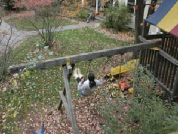
\includegraphics[width=.28\textwidth]{lag1.png}
  }\qquad
  \subfloat[特征点轨迹聚类]{%
    \label{fig:lag-cluster}
    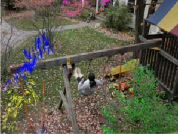
\includegraphics[width=.28\textwidth]{lag2.png}
  }\qquad
  \subfloat[分割动作层]{%
    \label{fig:lag-layers}
    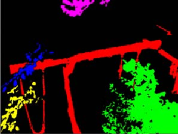
\includegraphics[width=.28\textwidth]{lag3.png}
  }\\
  \subfloat[直接放大(c)中秋千的动作层得到的结果(出现了空洞)]{%
    \label{fig:lag-motion-magnification}
    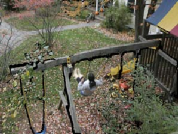
\includegraphics[width=.28\textwidth]{lag4.png}
  }\qquad
  \subfloat[对(d)进行背景填充得到的结果]{%
    \label{fig:lag-backgruond-fill}
    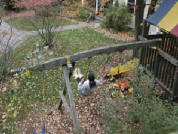
\includegraphics[width=.28\textwidth]{lag5.png}
  }\qquad
  \subfloat[先对(c)中秋千的动作层进行人工编辑再放大的结果]{%
    \label{fig:lag-modification}
    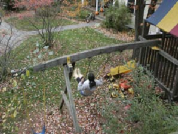
\includegraphics[width=.28\textwidth]{lag6.png}
  }
  \caption{拉格朗日视角的放大方法的处理流程}
  \label{fig:lag}
\end{figure}

图\ref{fig:liu}给出了使用文献\cite{liu2005motion}的方法对一个书架因受到按压
而发生的形变的放大结果。

\clearpage

\begin{figure}[htbp]
  \centering
  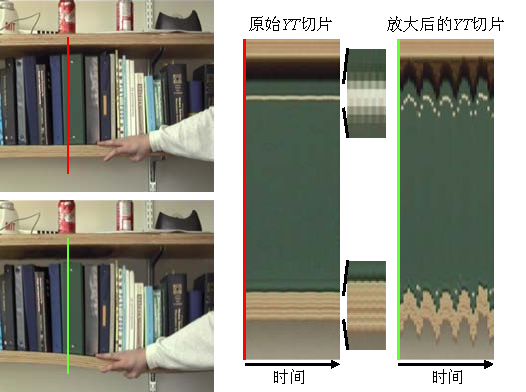
\includegraphics[width=.8\textwidth]{liu.pdf}
  \caption{使用拉格朗日视角的放大方法放大动作的结果}
  \label{fig:liu}
\end{figure}

拉格朗日视角的影像动作放大方法可以有效地从视频场景中找出微小的动作变化并进行放大。
然而,该方法存在以下几点不足:

\begin{compactenum}
\item 需要对特征点的运动轨迹进行精确的跟踪和估计。这个过程会耗费较多的计算资源。
\item 对特征点的跟踪容易受到遮挡的影响,从而影响跟踪结果。
\item 动作层分割的准确程度直接关系到最终的放大效果,而这个过程往往需要结合人工编
  辑才能达到理想的准确度,否则将导致放大结果出现空洞,需要在后期对图像进行背景
  填充等修补操作,这同样会增加算法的复杂度。
\end{compactenum}

\section{欧拉视角的影像动作放大方法}
\label{sec:eulerian}

欧拉视角的影像动作放大方法又被称为欧拉影像放大技术(Eulerian Video
Magnification, EVM)。2012 年,文献\cite{wu2012eulerian}提出了一种线性的欧拉影像动
作放大方法。其流程如下:

\begin{compactenum}
\item 空间域滤波。将视频序列进行金字塔多分辨率分解,得到不同空间频率的基带。
\item 频率滤波。对每个基带的图像进行频率域带通滤波,得到感兴趣的若干频带。
\item 动作放大。对带通滤波的结果进行线性放大。
\item 合成视频。合成经过放大后的图像。
\end{compactenum}

文献\cite{wu2012eulerian}的算法框架如图\ref{fig:linear}所示。

\begin{figure}[htbp]
  \centering
  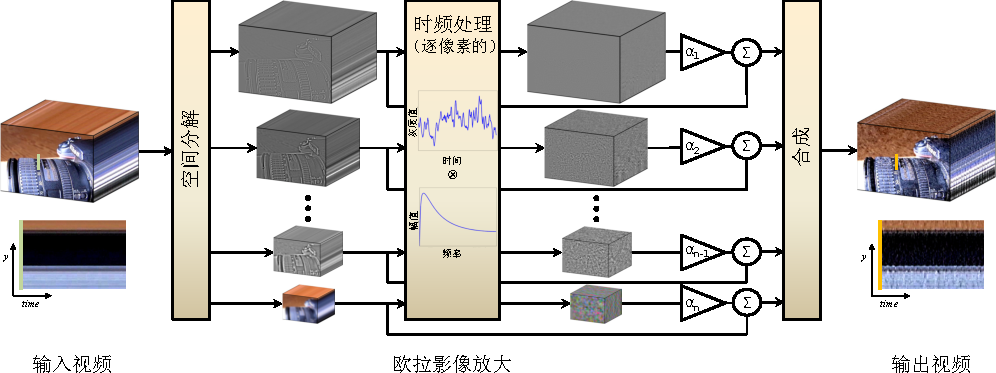
\includegraphics[width=1.1\textwidth]{linear.pdf}
  \caption{线性的欧拉影像动作放大方法的算法框架图}
  \label{fig:linear}
\end{figure}

与拉格朗日视角的方法相比,欧拉视角的动作放大方法运算速度快,无需对放大后的结果进
行背景填充。除此之外,该方法不仅可以用来放大动作的变化,还可以用来放大颜色的变化。
图\ref{fig:color-motion}分別给出了使用文献\cite{wu2012eulerian}的方法放大动作和
颜色变化的结果,每一行右侧的图片代表视频中某条竖线的$YT$切片,该竖线的位置如图
\ref{fig:color-motion-original}中最左侧子图的绿线所示。

\begin{figure}[htbp]
  \centering
    \subfloat[输入视频及$YT$切片]{%
      \label{fig:color-motion-original}
      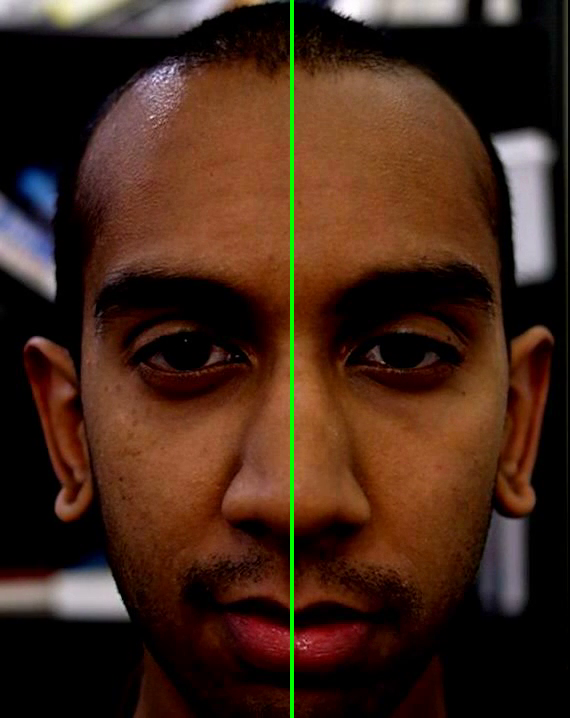
\includegraphics[height=2.5cm]{face2-1.png}~
      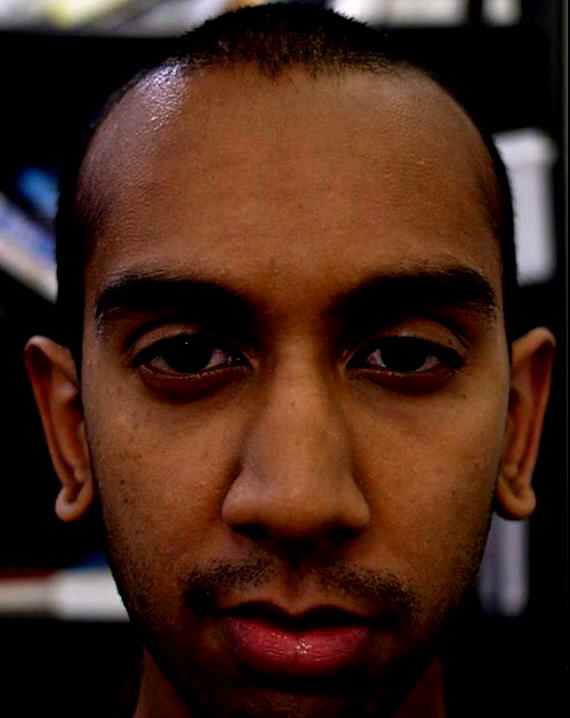
\includegraphics[height=2.5cm]{face2-3.png}~
      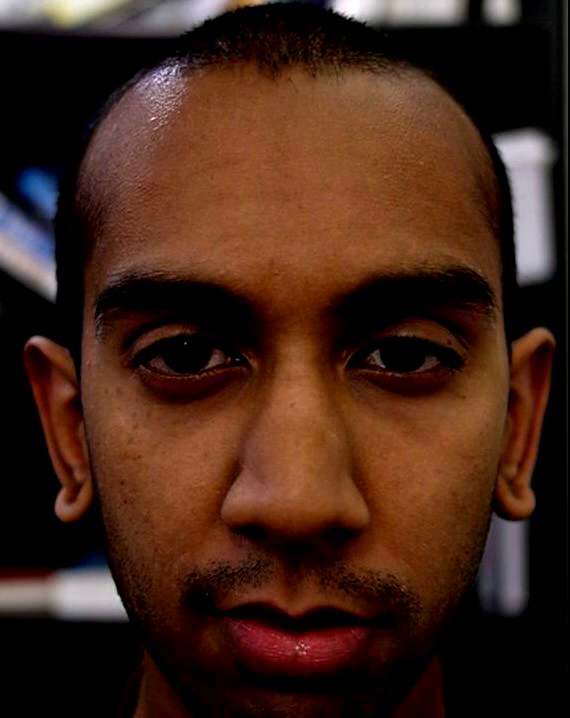
\includegraphics[height=2.5cm]{face2-4.png}~
      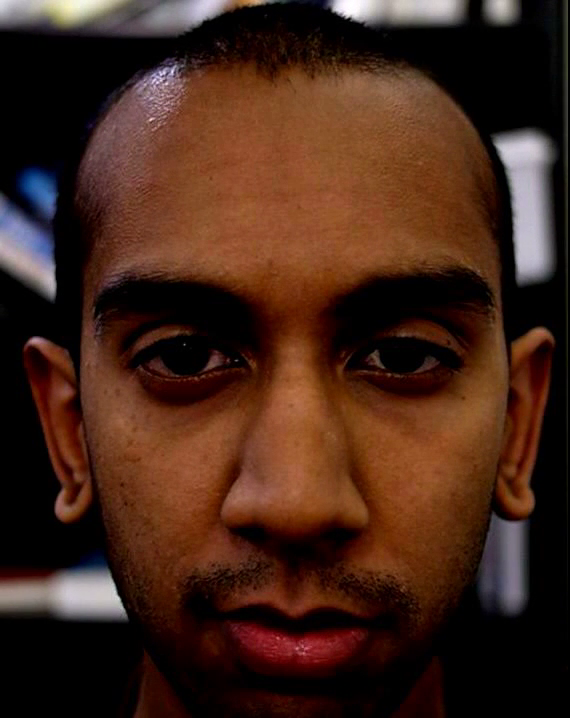
\includegraphics[height=2.5cm]{face2-5.png}\qquad
      \scalebox{4}[1]{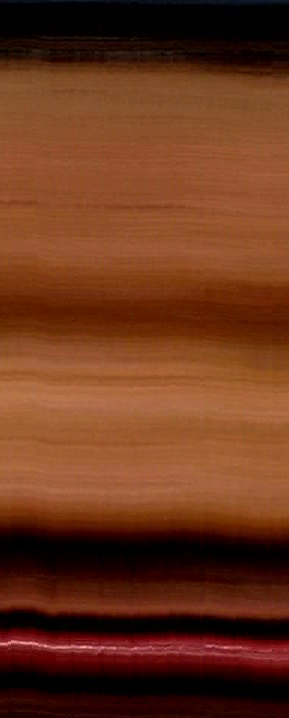
\includegraphics[height=2.5cm]{face2-slice.png}}
    }\\
    \subfloat[动作变化放大结果及$YT$切片]{%
      \label{fig:color-motion-motion}
      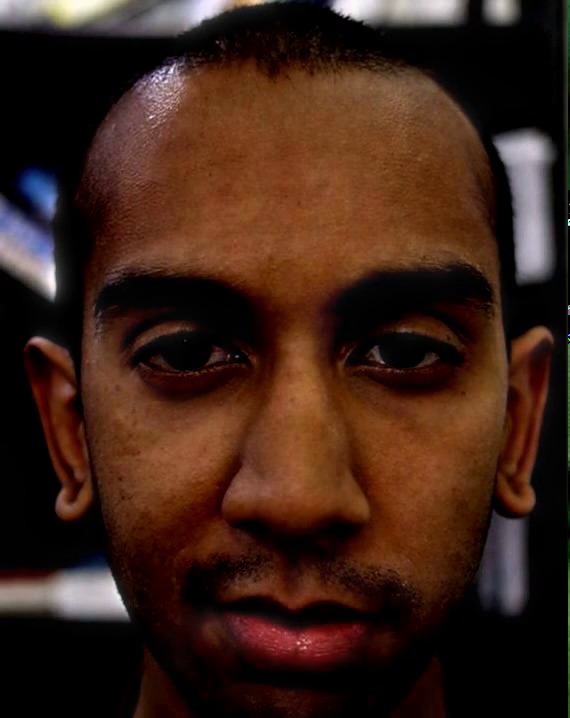
\includegraphics[height=2.5cm]{face2-motion-2.png}~
      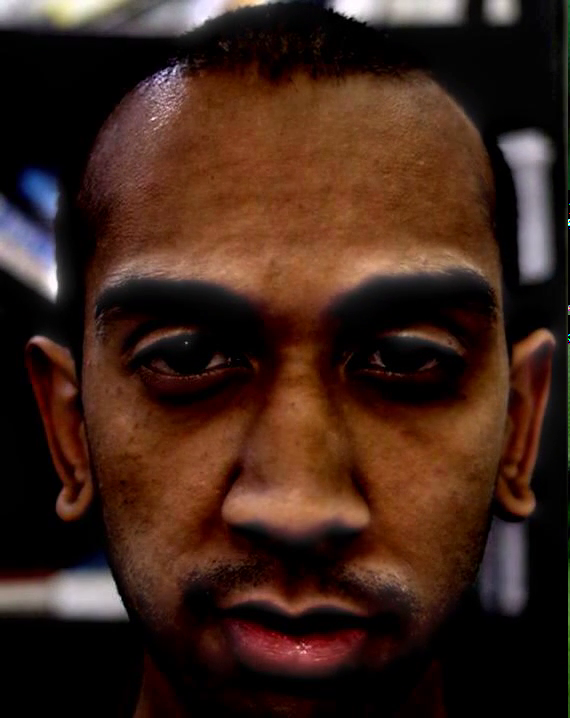
\includegraphics[height=2.5cm]{face2-motion-3.png}~
      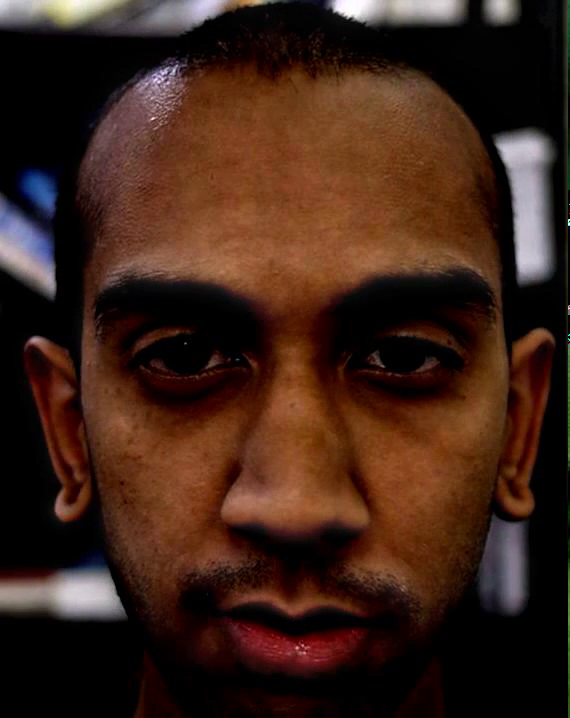
\includegraphics[height=2.5cm]{face2-motion-4.png}~
      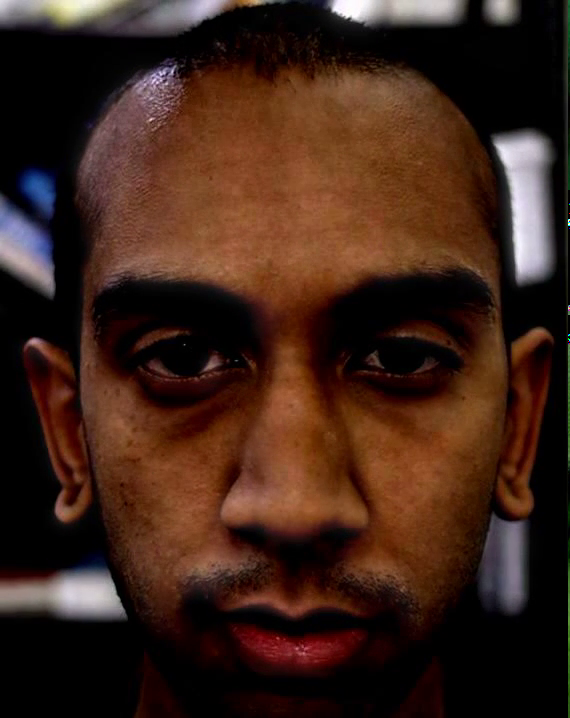
\includegraphics[height=2.5cm]{face2-motion-5.png}\qquad
      \scalebox{4}[1]{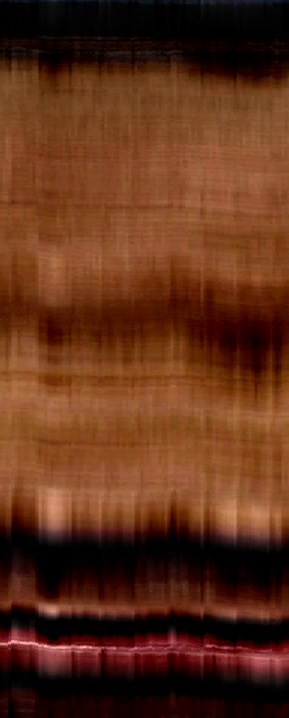
\includegraphics[height=2.5cm]{face2-motion-slice.png}}
      
    }\\
    \subfloat[颜色变化放大结果及$YT$切片]{%
      \label{fig:color-motion-color}
      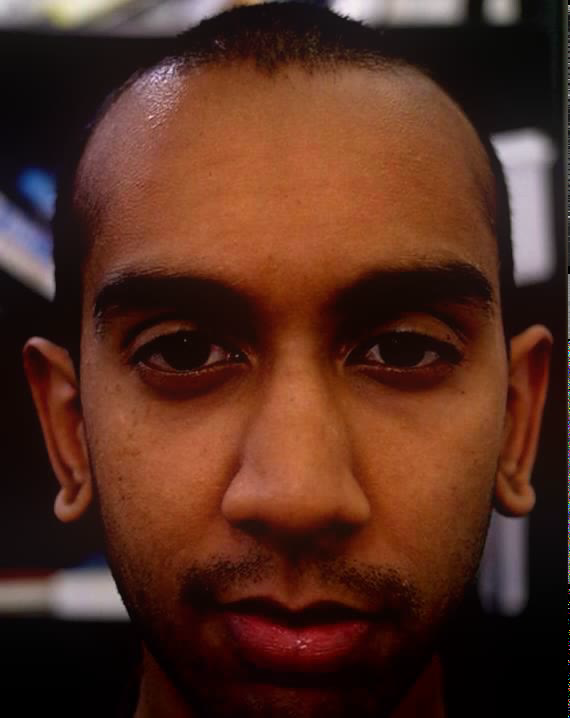
\includegraphics[height=2.5cm]{face2-color-2.png}~
      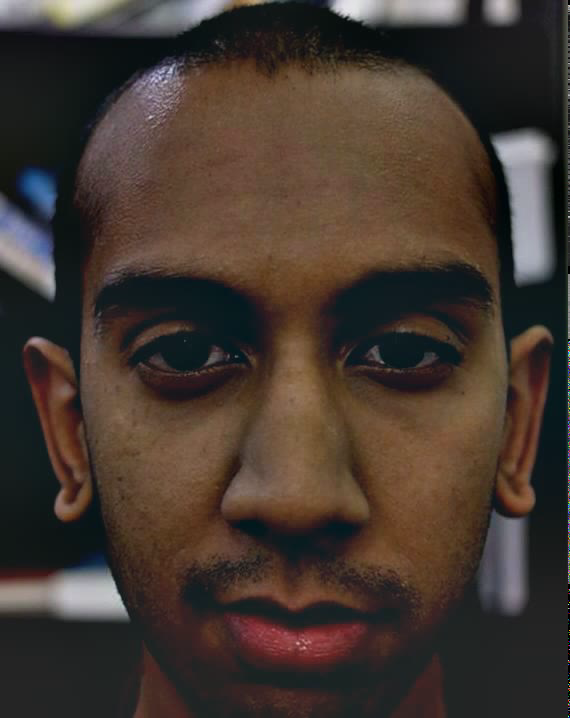
\includegraphics[height=2.5cm]{face2-color-3.png}~
      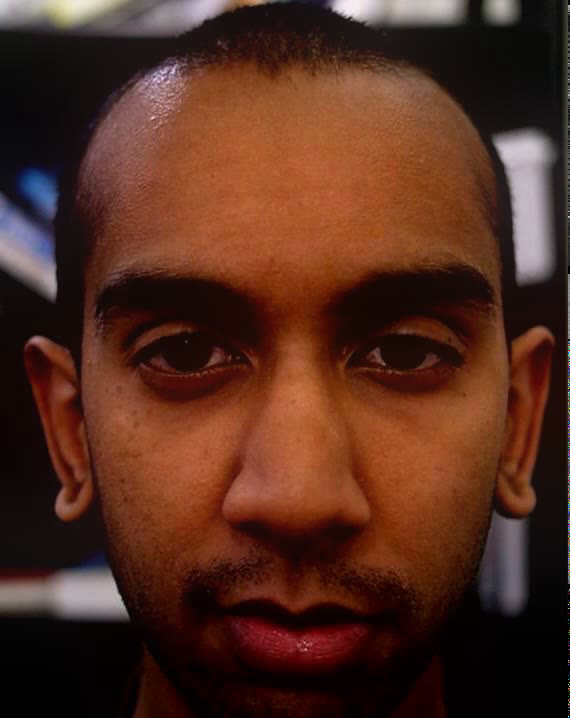
\includegraphics[height=2.5cm]{face2-color-4.png}~
      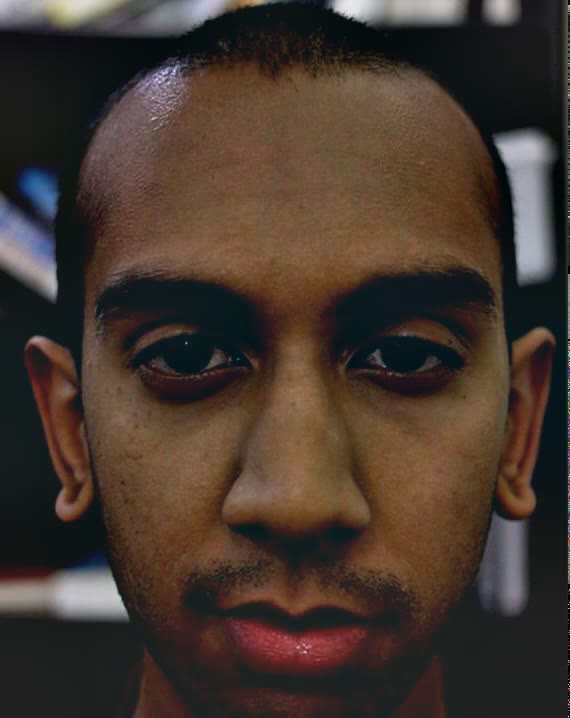
\includegraphics[height=2.5cm]{face2-color-5.png}\qquad
      \scalebox{4}[1]{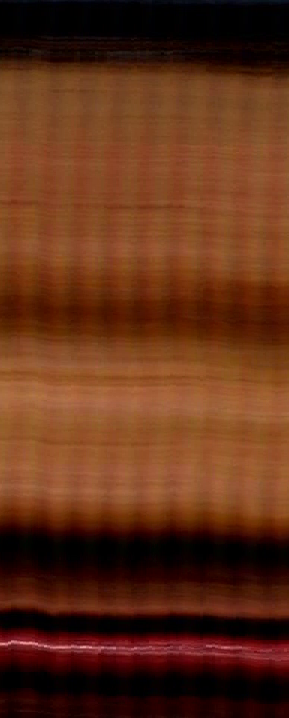
\includegraphics[height=2.5cm]{face2-color-slice.png}}
    }\\
  \caption{使用线性的欧拉影像动作放大方法放大动作变化和颜色变化的结果}
  \label{fig:color-motion}
\end{figure}

欧拉影像放大技术的第一步是对视频序列进行空间滤波。该过程主要借助拉普拉斯金字
塔\upcite{Burt1983},以分解得到不同的空间频率的基带。其原因有如下两点:

\begin{compactenum}
\item 有助于减少噪声。图像在不同空间频率下呈现出不同的信噪比(Signal to Noise
  Ratio, SNR)。空间频率越低,
  噪声越少,信噪比越高。因此,为了防止因放大噪声导致失真,可使用不同的放大倍数放
  大这些基带。最顶层的图像,即空间频率最低、信噪比最高的图像,可使用最大的放大倍
  数,下一层的放大倍数依次减小。
\item 便于对图像信号的逼近。空间频率较高的图像(如原视频图像)可能难以用泰勒级数
  展开来逼近。
\end{compactenum}

% 对视频序列的空间分解主要借助图像金字塔。如果要放大动作的变化,可以使用拉普拉斯金
% 字塔;如果要放大颜色的变化,则可以使用高斯金字塔。

得到不同空间频率的基带后,接下来需要对每一个基带进行频域的带通滤波,以得到感兴趣
的变化信号。

带通滤波器可以依据具体的应用来选择。窄通带的滤波器,如理想带通滤波器,可以直接截
取出感兴趣的频段,而避免放大其他频段,因而更适合用于需要对放大结果进行后续的时频
分析(例如提取心率、分析乐器的频率)的场合;宽通带的滤波器,如Butterworth带通滤波
器,二阶无限脉冲响应滤波器(Infinite Impulse Response Filter)等,可以更好的防止
振铃现象\cite{Gonzalez:2006:DIP:1076432},且更易于实现实时操作,因而更适合用在实
时性要求高,且不需要对放大结果进行时频分析的场合。

表\ref{tab:filters}列举了文献\cite{wu2012eulerian}处理face、guitar、subway及
wrist几个案例时所使用的滤波器。

\clearpage

\begin{table}[htbp]
  \centering
  \caption{文献\cite{wu2012eulerian}所使用的滤波器}
  \label{tab:filters}
  \begin{tabular}[c]{cccc}
    \toprule[1.5pt]
    案例名称 & 代表帧 & 滤波器示意图 \\
    \midrule
    face & \mgape{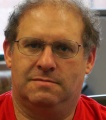
\includegraphics[height=3cm]{face.jpg}}
    & \mgape{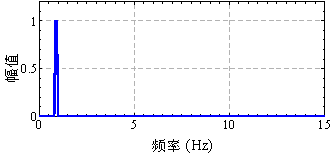
\includegraphics[height=3cm]{filter-face.pdf}} \\
    
    guitar & \mgape{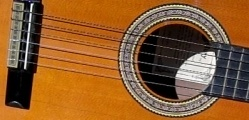
\includegraphics[height=2.6cm]{guitar.jpg}} &
    \mgape{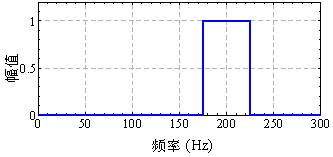
\includegraphics[height=3cm]{filter-guitar.pdf}}\\
    subway & \mgape{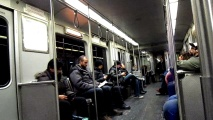
\includegraphics[height=3cm]{subway.jpg}} & 
    \mgape{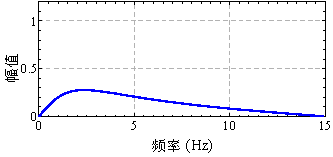
\includegraphics[height=3cm]{filter-subway.pdf}}\\
    wrist & \mgape{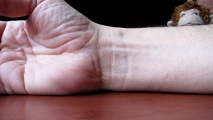
\includegraphics[height=3cm]{wrist.jpg}} &
    \mgape{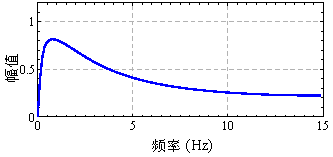
\includegraphics[height=3cm]{filter-wrist.pdf}}
    \\
    \bottomrule[1.5pt]
  \end{tabular}
\end{table}

文献\cite{wu2012eulerian}论证了带通滤波与感兴趣动作的关系:带通滤波的结果,就是对
感兴趣动作的逼近。

  以一维信号为例,设$I(x,t)$为点
$x$在$t$时刻的灰度值,且初始值为$f(x)$,则有:
\begin{equation}
  \label{eq:1}
  \left\{ \begin{aligned} I(x,t) & = f(x+\delta(t)) & , t >0 \\ I(x,0) & = f(x) &
        , t=0 \end{aligned} \right.
\end{equation}

其中,$\delta(t)$是变化信号。

要得到这个动作放大$\alpha$倍后的结果,就是要得到:

\begin{equation}
  \label{eq:2}
  \hat{I}(x,t)=f(x+(1+\alpha)\delta (t))
\end{equation}

为了将变化的部分分离出来,使用一阶泰勒级数展开来逼近公式\ref{eq:1}表示的动作:
\begin{equation}
  \label{eq:3}
  I(x,t)\approx f(x)+\delta(t)\frac{\partial f(x)}{\partial x}
\end{equation}

设上一步带通滤波的结果为$B(x,t)$,如果所有的变化信号$\delta(t)$的频率范围恰
好在带通滤波的频带范围之内,则有
\begin{equation}
  \label{eq:4}
  B(x,t)=\delta(t)\frac{\partial f(x)}{\partial x}
\end{equation}

对公式\ref{eq:2}所逼近的动作进行放大,就是将变化的部分乘以一个放大倍数
$\alpha$,再加回原来的信号中。即:
\begin{equation}
  \label{eq:5}
  \tilde{I}(x,t)=I(x,t)+\alpha B(x,t)
\end{equation}

联立公式\ref{eq:2}-\ref{eq:4},可得
\begin{equation}
  \label{eq:6}
  \tilde{I}(x,t)\approx f(x)+(1+\alpha)\delta(t)\frac{\partial f(x)}{\partial x}
\end{equation}

在这种情况下,$\tilde{I}(x,t)$约等于要求解的$I(x,t)$,即:
\begin{equation}
  \label{eq:7}
  \tilde{I}(x,t)\approx f(x+(1+\alpha)\delta(t))
\end{equation}

如果变化信号$\delta(t)$的频率范围超出了所选的频段范围。这种情况下,应用带通滤波
意味着只是保留了一部分的变化信号,而其他频率超出范围的信号将会被减弱。用$\gamma_k(t)$来表示在$t$时刻变化第$k$个变化信号减弱的倍数($0\le \gamma_k \le
1$),则有:
\begin{equation}
    \label{eq:8}
    B(x,t) = \sum_k \gamma_{k}\delta_{k}(t)\frac{\partial f(x)}{\partial x}
\end{equation}

此时,动作的放大可以用公式\ref{eq:9}表示:
\begin{equation}
  \label{eq:9}
  \tilde {I}(x,t)\approx f(x+\sum_k(1+\alpha_{k})\delta_{k}(t))
\end{equation}

其中,$\alpha_k$是$\alpha$与$\gamma_{k}$的乘积。

图\ref{fig:sinusoid}演示了对一个正弦信号的逼近和放大过程。

\begin{figure}[htbp]
  \centering
  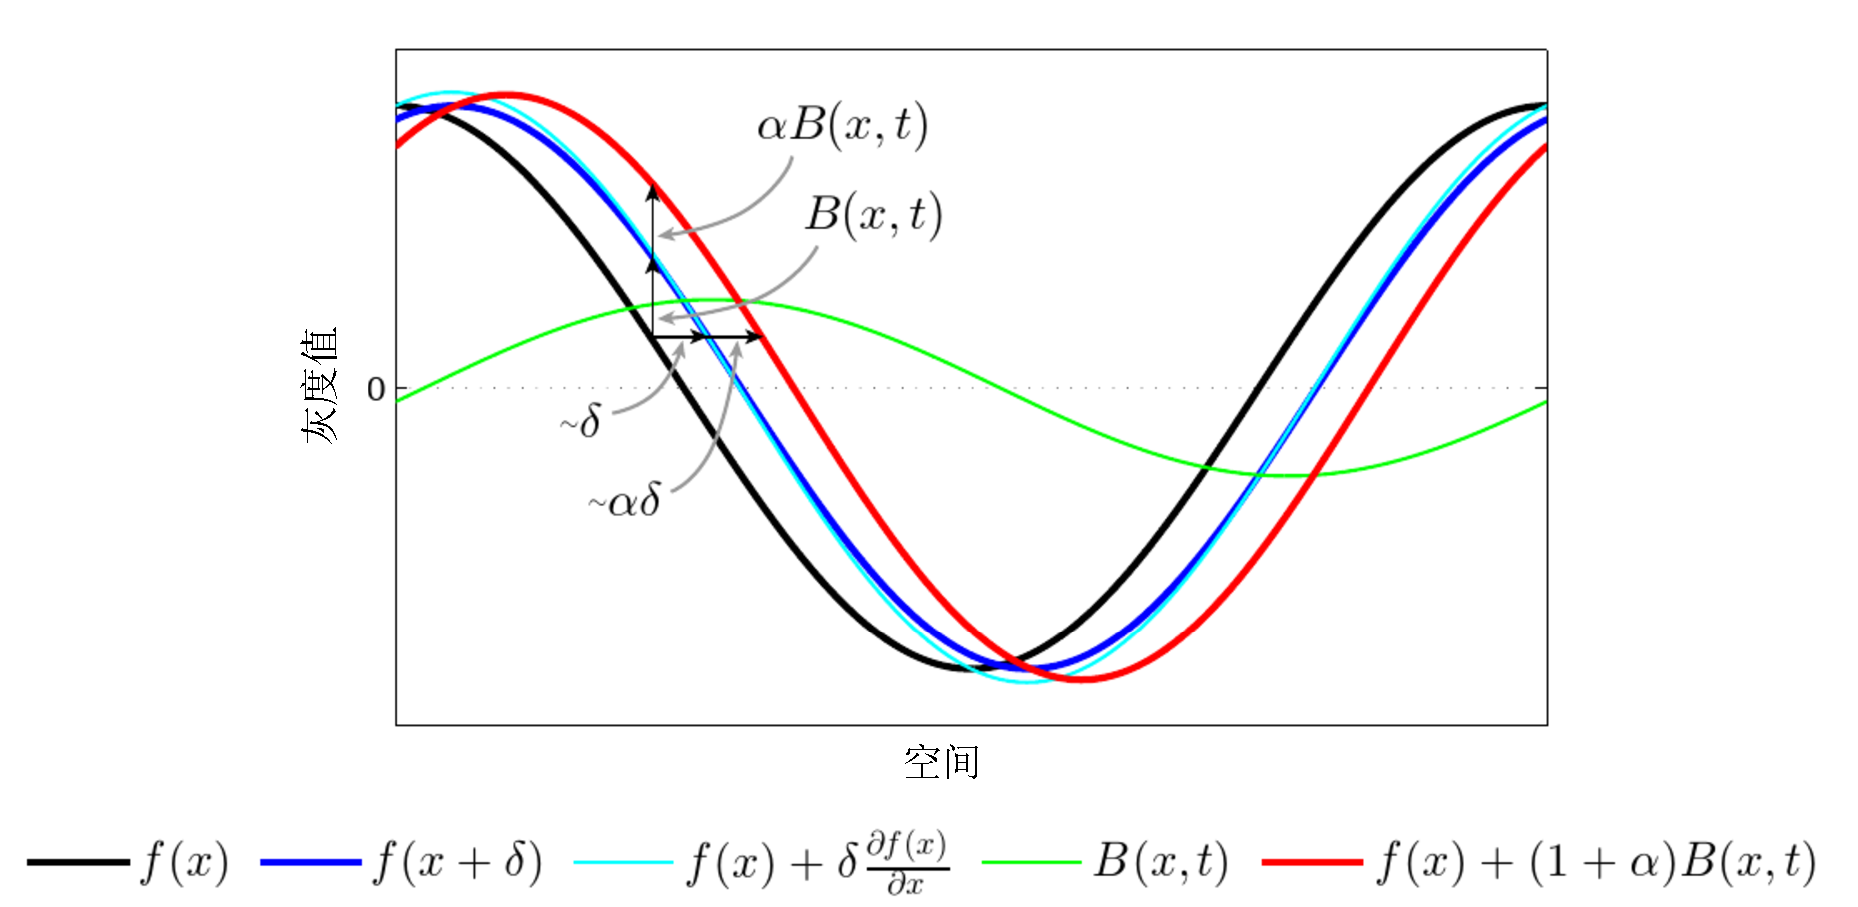
\includegraphics[width=\textwidth]{sinusoid.pdf}
  \caption{对一个正弦信号的逼近和放大过程}
  \label{fig:sinusoid}
\end{figure}

以上关于带通滤波结果与动作的关系结论是建立在相对平滑的图像和小的动作信号的假设上
的。对于空间频率较高的图像,使用泰勒级数逼近的结果会产生较大误差。文献
\cite{wu2012eulerian}给出了当前基带的空间频率$\omega$与放大倍数的界限值:
\begin{equation}
  \label{eq:bound1}
  (1+\alpha)\delta(t)<\frac{\lambda}{8}
\end{equation}

其中,$\lambda$是当前基带的空间波长,即$\lambda=\frac{\pi}{\omega}$。公式
\ref{eq:bound1}提供了计算每一层基带的合理放大倍数的准则。如图\ref{fig:guide}
所示,当$\alpha$达到该界限时,就维持在该界限值。

\clearpage

\begin{figure}[htbp]
  \centering
  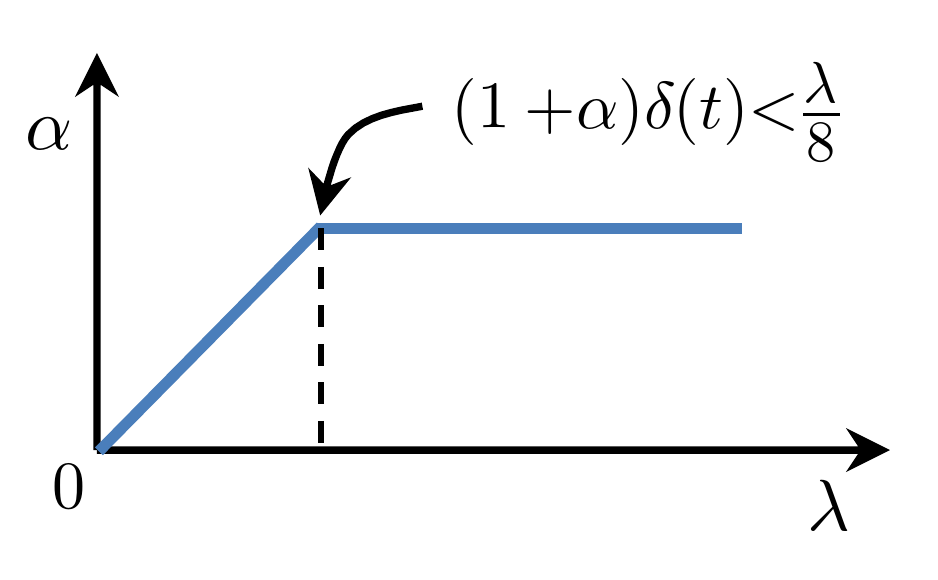
\includegraphics[width=6.5cm]{guide.png}
  \caption{放大倍数$\alpha$的界限值}
  \label{fig:guide}
\end{figure}

线性的欧拉影像动作放大方法会在放大动作的同时放大噪声,所允许的放大倍数也较小。
2013年,文献\cite{Wadhwa2013PhaseBased}提出了一种基于相位的改进算法——首先使用抗混淆的复值可
控金字
塔
\upcite{portilla2000parametric,simoncelli1992shiftable,simoncelli1995steerable}来
进行多分辨率分解,并受到基于相位的光流
法\upcite{gautama2002phase,fleet1990computation,freeman1991motion}的启发,通过分
离和操纵滤波后信号的相位来调整动作的幅度。其流程如下:

\begin{compactenum}
\item 空间滤波。使用复值可控金字塔进行空间域分解,得到每个尺度、每个方向和位置的相位图。
\item 带通滤波。对每个尺度、每个方向和位置的信号进行带通滤波,得到感兴趣的若干频
  带,并去除直流分量。
\item 动作放大。放大带通滤波的结果。
\item 合成视频。合成经过放大的图像。
\end{compactenum}

基于相位的欧拉影像动作放大方法的算法框架如图\ref{fig:phase}所示。

\begin{figure}[htbp]
  \centering
  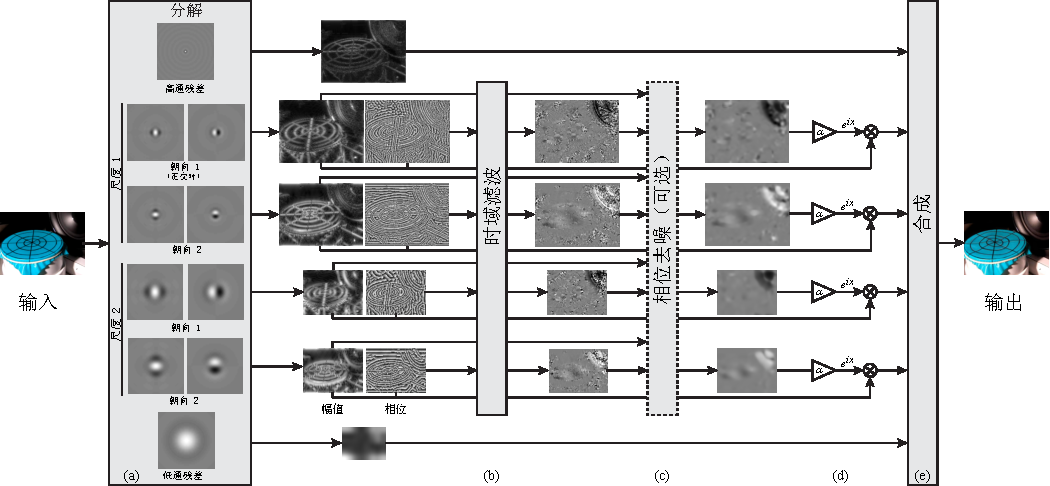
\includegraphics[width=1.1\textwidth]{phase.pdf}
  \caption{基于相位的欧拉影像动作放大方法的算法框架图}
  \label{fig:phase}
\end{figure}

基于相位的欧拉影像放大技术在放大动作的同时不会放大噪声,而是平移了噪声,因此允许
更大的放大倍数,其界限为
\begin{equation}
  \label{eq:bound2}
  a\delta(t)<\lambda \frac{n}{4}
\end{equation}

其中,$n$为复值可控金字塔的方向基带每个倍频程的滤波器数量。

图\ref{fig:compare}给出了分别使用两种方法放大一个吊车受风吹动产生的形变的结果对比。

\begin{figure}[htbp]
  \centering
  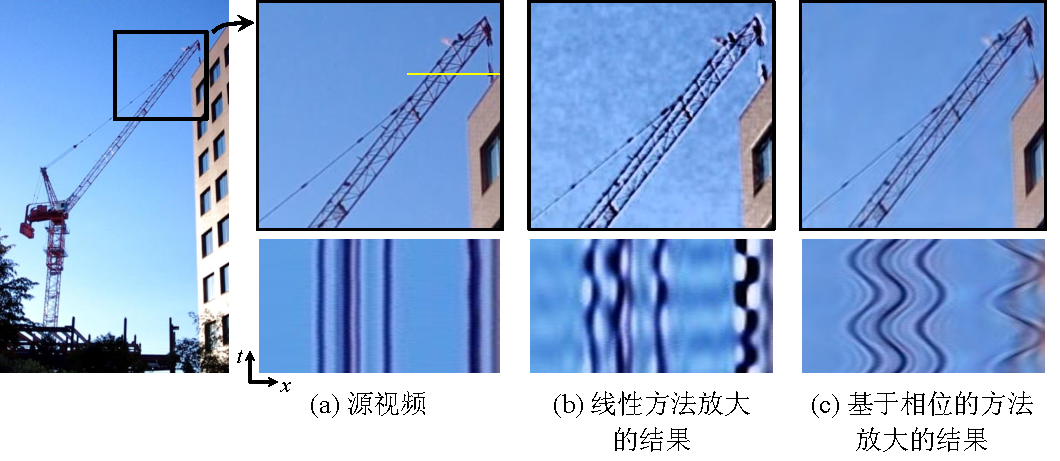
\includegraphics[width=\textwidth]{compare.pdf}
  \caption{线性的基于相位的欧拉影像放大方法的结果对比图。
    %(a) 顶部图:吊车的局部放大图。底部图:顶部图黄线区域的像素值随时
    %间变换的$XT$截面图。(b) 线性的方法的放大结果。噪声会连同吊车的动作一起被放
    %大,从而导致较大失真。(c) 基于相位的方法的放大结果,该方法在使用较大的放大倍
    %数时仍然不会引入较大噪声。
  }
  \label{fig:compare}
\end{figure}

欧拉影像动作放大方法的不足之处在于其分析的是整个场景中的感兴趣频段,对于存在大幅
度动作的场景,带通滤波的结果并不能反映真实的动作信息,此时的放大结果会产生明显
的“鬼影”现象,从而影响放大效果,如图\ref{fig:large-motion}所示。此外,对场景
中的非感兴趣区域的放大也会影响对放大结果的后继分析,如心率提取等。

\clearpage

\begin{figure}[htbp]
  \centering
  \subfloat[线性的方法]{%
      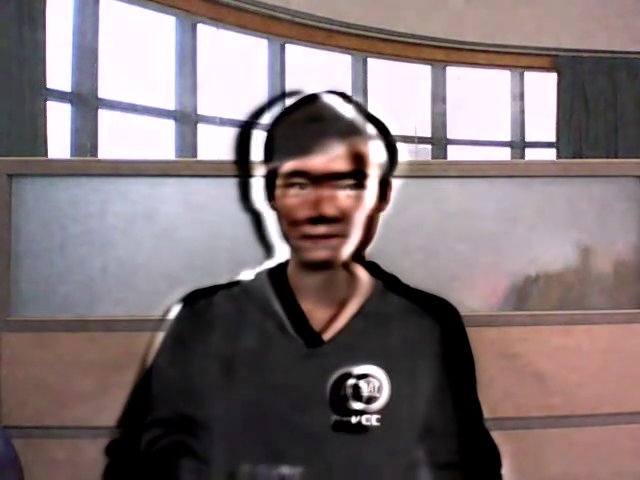
\includegraphics[width=.45\textwidth]{ghost-linear.png}
    }\qquad
   \subfloat[基于相位的方法]{%
      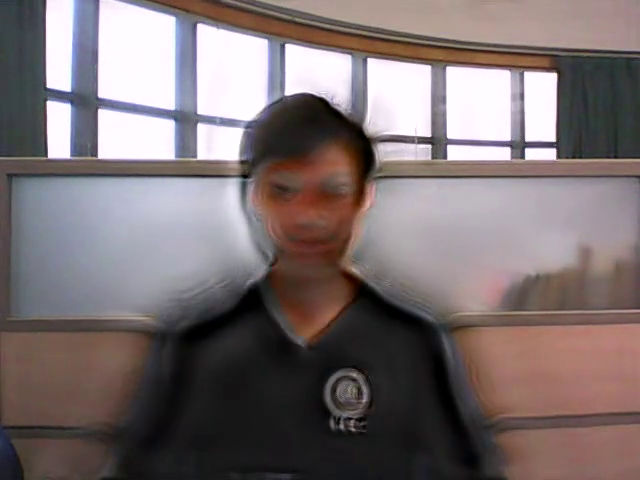
\includegraphics[width=.45\textwidth]{ghost-phase.png}
    }
  \caption{欧拉影像动作放大方法直接放大存在大幅度动作的场景会导致“鬼影”现象}
  \label{fig:large-motion}
\end{figure}

对于这个问题,文献\cite{Wadhwa2013PhaseBased}将相位的变化幅度超过一个阈值的动作
的放大倍数都设为0来避免对这些区域进行放大。如图\ref{fig:ignore}所示。

\begin{figure}[htbp]
  \centering
  \subfloat[直接全局放大结果,存在明显失真]{%
      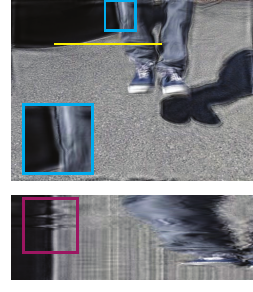
\includegraphics[width=.45\textwidth]{ignore.pdf}
    }~
   \subfloat[不对存在大幅度动作的物体进行放大]{%
      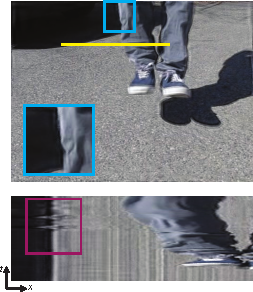
\includegraphics[width=.45\textwidth]{ignore2.pdf}
    }
  \caption{文献\cite{Wadhwa2013PhaseBased}通过避免放大存在大幅度动作的物体来防止失真}
  \label{fig:ignore}
\end{figure}

然而,这个方法直接忽略了存在大幅度动作的物体,因而无法对大幅度动作中的物体的细节
变化进行放大。而这类需求在实际生活中普遍存在,如放大一个移动中的人的脸部表情、颜
色变化等,显然上述的策略无法适应这类需求。

%%% Local Variables: 
%%% mode: latex
%%% TeX-master: "../thesis"
%%% End: 

\chapter{前景约束的欧拉影像动作放大技术}
\label{chap:fc-evm}

针对第\ref{chap:previous}章中所介绍的几种动作放大方法的不足,本文提出一种前景约束
的欧拉影像动作放大方法,该方法在欧拉视角的动作放大方法的基础上,结合了拉格朗日视
角的特点,通过使用目标跟踪技术,将放大区域限制在由用户选定的感兴趣区域上,再通过
使用前景分割技术,将动作放大结果与原图像进行金字塔混合,将放大区域进一步限制在感
兴趣区域中的前景区域。数学上,本文使用四元数矩阵一次性处理视频的彩色序列帧的三个
通道,具备更好的完整性。

本文的算法包括如下几个步骤:

\begin{compactenum}
\item 选择感兴趣区域(Region of Interest,ROI)。用户在参照帧中手动框选一个感兴
  趣的区域(如人脸),作为后续的跟踪目标和前景分割的标注区域。
\item 区域跟踪和前景提取。使用目标跟踪算法对感兴趣区域进行跟踪,并从跟踪区域中提取出前景掩码。
\item 局部欧拉影像动作放大。对跟踪区域进行局部的欧拉影像动作放大。
\item 金字塔率混合。将放大结果与区域原图进行金字塔混合。
\item 合成视频。合成最终视频。
\end{compactenum}

本文的算法框架如图\ref{fig:fc-evm-frameworks}所示。出于论述上的简单,本文主要采
用线性的欧拉影像动作放大算法进行动作放大。该算法也可以直接替换成基于相位的方法,
以得到最优的放大结果。

\begin{landscape}
  \begin{figure}[htbp]
  \centering
  \scalebox{1.5}[1.5]{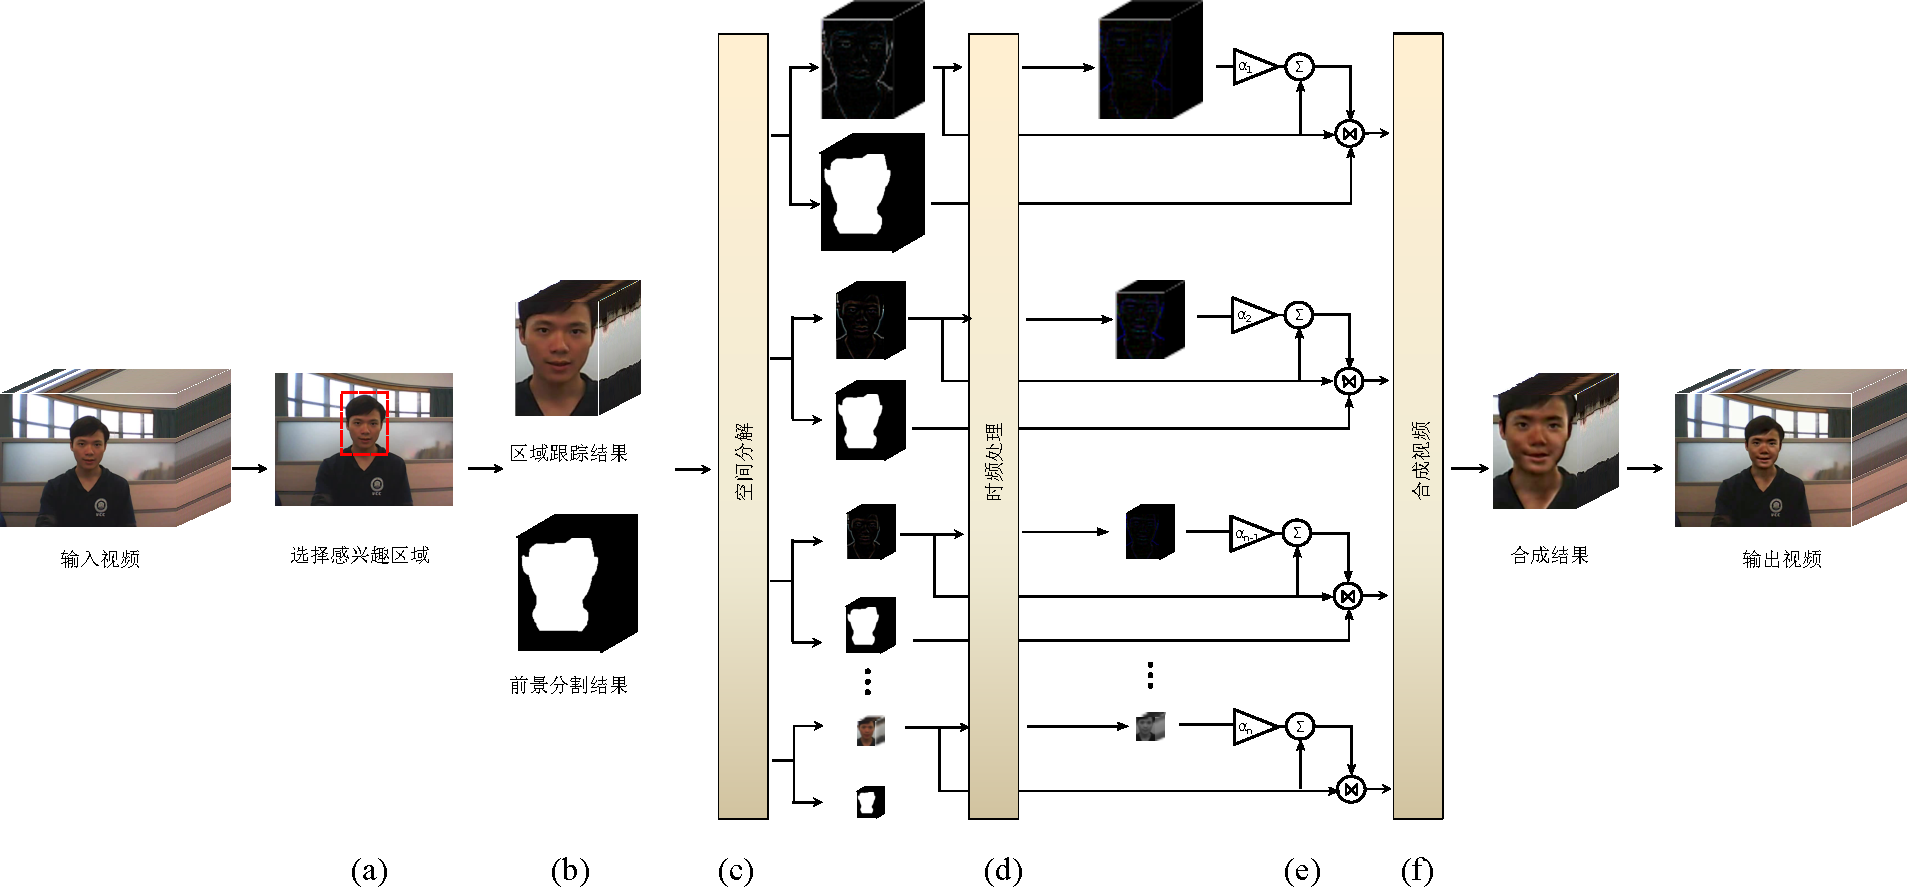
\includegraphics[width=\textwidth]{fc-evm.pdf}}
  \caption{前景约束的欧拉动作放大算法框架图。(a) 读入视频后,用户在参照帧中框选一
    个感兴趣的区域;(b) 根据用户选定的区域,对每一帧进行区域跟踪,同时使用前景分
    割技术分割出与区域大小相同的前景掩码;(c) 将每一帧跟踪到的区域图像和前景掩码
    分别分解成$n$层的拉普拉斯金字塔和高斯金字塔;(d) 对区域图像的每一层基带进行
    带通滤波;(e) 根据当前的空间频率,使用一个合理的放大倍数$\alpha_i$对滤波结
    果进行放大。将放大结果与原图进行叠加后,再利用前景掩码与原图进行一次金字塔混
    合;(f) 最后合成视频。}
  \label{fig:fc-evm-frameworks}
\end{figure}
\end{landscape}

\section{区域跟踪}
\label{sec:tracking}

为了放大存在大幅度动作的物体中的细微变化,算法先对该物体中的感兴趣区域进行
目标跟踪,以方便后期使用欧拉影像动作放大方法对跟踪结果进行放大。在开始跟踪前,首
先要求用户在参照帧中框选出感兴趣区域,这个区域将有两个用途:

\begin{compactenum}
\item 作为区域跟踪的目标区域。
\item 作为前景分割的标注区域。
\end{compactenum}

用户确定好感兴趣区域后,本文使用文献\cite{常发亮2007}提出的Mean-shift跟踪
与Kalman滤波相结合的算法对视频中的每一帧进行区域跟踪,以找出与感兴趣区域最相似的
目标候选区域。该算法在目标受到干扰和遮挡的情况下依然能够具有较好的跟踪效果。

\subsection{Mean-shift算法}
\label{sec:mean-shift}

Mean-shift算法是一种在一组数据的密度分布中寻找局部极值的算
法\upcite{comaniciu2002mean,fukunaga1975estimation},该算法利用可视化特征(如颜色、
纹理等)的统计信息描述跟踪的目标,并通过梯度下降策略,找出与目标模式具有最大相似
度的目标候选区域作为跟踪结果。

为了从彩色图像中得到目标模式,算法首先将图像由RGB色彩空间转换到HSV色彩空间,
之后提取出Hue分量,并将其分成$m$等份,每一等份对应一个子特征值,则第$u$个特
征值的概率分布为\upcite{duda1973pattern}:
\begin{equation}
  \label{eq:characteristic-prob}
  q_{u}=C\sum_{i=1}^{n}k\left( \left\| \frac{x_{0}-x_{i}}{h} \right\|^{2}
  \right)\delta[b(x_{i})-u],\qquad i\in[1,\ldots,n]
\end{equation}

其中,$x_{0}$ 是搜索窗口的中心点的位置,$x_{i}$ 是窗口内第$i$点的位置,
$k\left( \left\| x \right\|^{2} \right)$ 是核函数,$h$ 是窗宽。$b$ 为脉冲函数,
用于保证只有第$u$个特征值的像素才能对概率分布作出贡献。$\delta$为Kronecker
delta函数。归一化常数$C$用于保证$\sum_{u=1}^{m}\hat{q_u}=1$。

目标候选模式的核直方图计算方法与公式\ref{eq:characteristic-prob}类似。假设$y_0$是当前帧的目标候选区域的中心点,则其概率分布为:
\begin{equation}
  \label{eq:target-candidate}
  p_{u}(y_0)=C\sum_{i=1}^{n}k\left( \left\| \frac{y_{0}-x_{i}}{h} \right\|^{2}
  \right)\delta[b(x_{i})-u],\qquad i\in[1,\ldots,n]
\end{equation}

引入Bhattacharyya系数来衡量目标模式与目标候选模式的相似度:
\begin{equation}
  \label{eq:Bhattacharyya}
  \rho(\rho(y),q)=\sum_{u=1}^{m}\sqrt{p_{u}(y)q_{u}}
\end{equation}

对于两个颜色分布直方图的匹配,可以定义如下的距离公式,计算两个分布之间的距离:
\begin{equation}
  \label{eq:distance}
  d(y)=\sqrt{1-\rho(y)}
\end{equation}

$d(y)$ 越小,两个颜色分布直方图越相近。

在搜索阶段,算法使用梯度下降的策略搜索使Bhattacharyya系数达到最大的目标候选区
域。对$\rho(\rho(y),q)$进行泰勒级数展开可得:
\begin{equation}
  \label{eq:taylor}
  \rho(\rho(y),q)\approx \frac{1}{2}\sum_{u=1}^{m}\sqrt{p_u(y_0)q_u}+\frac{C}{2}\sum_{u=1}^{m}w_{i}k(\left\|y-x_i\right\|^2)
\end{equation}

其中,
\begin{equation}
    \label{eq:weight}
    w_{i}=\sum_{i=1}^{m}\sqrt{\frac{q_u}{p_{u}(y_0)}}\delta[b(x)-u]
\end{equation}

要使Bhattacharyya系数最大,即是使公式\ref{eq:taylor}的第二项达到最大。
因此,可沿梯度方向确定下一个目标候选区域的位置:
\begin{equation}
    \label{eq:next-position}
    y_{i}=\frac{\sum_{i=1}^{m}x_{i}w_{i}g\left(\left\|\frac{y_0-x_i}{h}\right\|^{2}\right)}{\sum_{i=1}^{m}w_{i}g\left(\left\|\frac{y_0-x_i}{h}\right\|^{2}\right)}
  \end{equation}

Mean-shift的搜索过程如算法\ref{alg:delta}所示。

\begin{algorithm}[htbp]
  \caption{Mean-shift搜索算法}
  \label{alg:delta}
  \begin{algorithmic}[1]
    \REQUIRE 目标模式$q_u$及上一帧的目标窗口的位置$y_0$ 。
    \STATE 初始化当前帧的搜索窗口为$y_0$,根据公
    式\ref{eq:target-candidate}计算$p_u(y_0)$,根据公式
   \ref{eq:Bhattacharyya}评估$\rho(\rho(y_0),q)$。
    \STATE 根据公式\ref{eq:weight}计算每一点的权值$w_{i}$ 。
    \STATE 根据公式\ref{eq:next-position}计算下一个目标候选区域的位置$y_{i}$
   。
    \STATE 根据公式\ref{eq:target-candidate}计算$p_u(y_1)$ ,根据公式
   \ref{eq:Bhattacharyya}评估$\rho(\rho(y_1),q)$。
    \STATE 如果$\left\|y_{i}-y_{0}\right\|$小于一个目标值$\varepsilon$,或者
    迭代次数超过了预先设定的最大迭代次数,则结束迭代;\\
    否则,令$y_{0}\leftarrow y_{i}$,返回步骤 2。
  \end{algorithmic}
\end{algorithm}
\par

\subsection{Kalman滤波}
\label{sec:kalman}

Kalman滤波又称为线性二次估计(Linear Quadratic Estimation, LQE),该方法能够
从一系列的不完全的,包含噪声的测量中预测目标的运动位置和速度。

Kalman 滤波包含两个模型:

\begin{compactenum}
\item 状态方程:
  \begin{equation}
    \label{eq:state}
    X_{k}=F\cdot X_{k-1}+W_k
  \end{equation}
\item 观测方程:
  \begin{equation}
    \label{eq:observation}
    Z_{k}=H\cdot X_{k}+K_{k}
  \end{equation}
\end{compactenum}

其中,$X_k = [x,y,dx,dy]^{T}$是系统在$k$时刻的状态向量,$x$和$dx$分别是水平
方向的位置和速度,$y$和$dy$则分别是竖直方向的位置和速度。$Z_k=[x,y]^{T}$是
系统在$k$时刻的观测向量,表示观测目标的位置。$W_k$和$V_k$分别为状态和观测对
应的高斯噪声向量,其方差矩阵分别为$Q$和$R$。$F$为状态转移矩阵,$H$为观测矩阵。
四个矩阵的值分别为\upcite{Zhang2009}:$$F=\begin{bmatrix}
  1 & 0 & 1 & 0\\0 & 1 & 0 & 1 \\ 0 & 0 & 1 & 0\\ 0 & 0 & 0 & 1
\end{bmatrix}
\mbox{,}~
H = \begin{bmatrix}
  1 & 0 & 0 & 0\\0 & 1 & 0 & 0
\end{bmatrix}
\mbox{,}~
Q=\begin{bmatrix}
  1 & 0 & 0 & 0\\0 & 1 & 0 & 0 \\ 0 & 0 & 1 & 0\\ 0 & 0 & 0 & 1
\end{bmatrix}
\mbox{,}~
R = \begin{bmatrix}
  1 & 0 \\0 & 1 
\end{bmatrix}
$$

给定一组观测向量$Z_1, Z_2, \ldots, Z_k$,Kalman滤波通过计算最小误差方差获得对
状态向量$X_k$的估计。过程如算法\ref{alg:kalman}所示。

\begin{algorithm}[htbp]
  \caption{Kalman 滤波}
  \label{alg:kalman}
  \begin{algorithmic}[1]
    \STATE 初始化:
    \begin{eqnarray*}
      \hat{X}_0&=&E[X_0]\\
      P_0&=&E[(X_0-E[X_0])(X_0-E[X_0])^{T}]
    \end{eqnarray*}
    \STATE 预测:
    \begin{eqnarray*}
      \hat{X}_{k+1,k}&=&F \hat{X}_{k}\\ 
      P_{k+1,k}&=&F P_{k}F^{T}+Q\\
      K_{k+1}&=&P_{k+1,k}H^{T}(H P_{k+1,k}H^{T}+R)^{-1}
    \end{eqnarray*}
    \STATE 估计:
    \begin{eqnarray*}
      \hat{X}_{k+1}&=&\hat{X}_{k+1,k}+K(Z_{k+1}-H\hat{X}_{k+1,k})\\
      P_{k+1}&=&(I-K_{k+1}H)P_{k+1,k}
    \end{eqnarray*}
  \end{algorithmic}
\end{algorithm}

其中,$\hat{X}_{k+1, k}$为状态向量的一步预测,$\hat{X}_{k+1}$为最优的状态估
计,$K_{k+1}$为滤波增益矩阵,$P_{k+1, k}$为一步预测误差方差阵,$P_{k+1}$为估计误
差方差阵。

\subsection{Mean-shift与Kalman滤波相结合的跟踪算法}
\label{sec:combine}

将Mean-shift跟踪算法与Kalman滤波相结合,可以在跟踪的过程中同时考虑目标的运动
方向和速度信息,从而较为稳定地跟踪场景中的目标。该算法对遮挡、光线变化等影响不敏
感。

$k+1$时刻目标的位置$\hat{X}_{k+1}$由式\ref{eq:target-pos}得到:
\begin{equation}
  \label{eq:target-pos}
  \hat{X}_{k+1}=\sigma \hat{X}_{k+1,k}+(1-\sigma)y_1
\end{equation}

其中,$\hat{X}_{k+1,k}$是由Kalman滤波预测的目标位置,$y_1$是Mean-shift跟踪
得到的目标位置。$\sigma$是一个比例因子($0 \le \sigma \le 1$),可以根据受干扰程
度取不同的值。目标跟踪过程中的受干扰程度可以使用Bhattacharyya系数来衡量:如果该
系数较大,表明目标受干扰程度较小,此时使用Mean-shift可以获得较好的跟踪结果,因
此可以取较小的$\sigma$值;反之,如果该系数较小,表明当前场景存在遮挡或光照变化
等干扰因素,此时应该增大Kalman滤波结果的比例,因此可以取较大的$\sigma$值。

结合了Mean-shift和Kalman滤波的跟踪算法步骤如算法\ref{alg:combine}所示。

\begin{algorithm}
  \caption{Mean-shift和Kalman滤波相结合的跟踪算法}
  \label{alg:combine}
  \begin{algorithmic}[1]
    \STATE 初始化目标的位置和速度;
    \STATE 使用Kalman预测目标在当前帧的位置$\hat{X}_{k+1,k}$;
    \STATE 使用Mean-shift算法获得目标在当前帧的位置$y_1$;
    \STATE 根据公式\ref{eq:Bhattacharyya}计算Bhattacharyya系数的值,选择合适
    的$\sigma$值,再根据公式\ref{eq:target-pos}计算目标位置$\hat{X}_{k+1}$ 。
  \end{algorithmic}
\end{algorithm}

\section{前景分割}
\label{sec:grabcut}

对感兴趣区域进行跟踪后,可以得到由目标区域的图像组成的新序列。此时,如果直接对该
序列进行欧拉影像动作放大,该区域中的背景部分的动作也会连同一块放大,导致最后的合
成结果在区域边缘出现明显的边界,如图\ref{fig:bound-artifact}所示。

\begin{figure}[htbp]
  \centering
  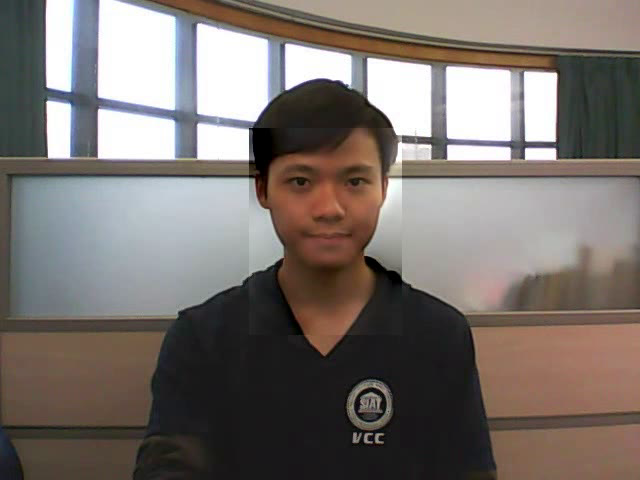
\includegraphics[width=.6\textwidth]{bound-artifact.png}
  \caption{直接对跟踪区域进行动作放大会导致区域边缘出现明显边界}
  \label{fig:bound-artifact}
\end{figure}

为了解决这个问题,本文在进行目标跟踪的同时,使
用GrabCut算法\upcite{Rother2004}从原视频图像帧中提取出目标区域的前景掩码。

GrabCut算法是在Graph Cuts算法的基础上发展而来的一种简单直观的分割算法,其与
Graph Cuts的区别在于:

\begin{compactenum}
\item 混合高斯模型(Gaussian Mixture Model,GMM)。Graph Cut使用灰度直方图作为目
  标和背景的模型,而GrabCut则使用RGB三通道的混合高斯模型。
\item 迭代估计(iterative estimation)。Graph Cuts算法是基于能量最小化一次性完成
  分割的,而GrabCut算法则是一个不断进行分割估计和模型参数学习的迭代过程。
\item 不完全标注(incomplete labelling)。Graph Cuts要求用户在目标和背景中选取一
  些种子点,因而需要较多的交互;而GrabCut只需要用户简单地框选包含目标的区域,就
  足以达到良好的分割效果。
\end{compactenum}

GrabCut的以上几点特性,尤其是不完全标注的特性,使其非常适合用在对目标区域中的前
景区域的进一步分割上:对每帧图像进行区域跟踪所得到的目标区域可以同时作
为GrabCut算法的标注区域。因此,本文的整个算法过程只需用户在参照帧框选一次感兴趣
区域,其他过程都可以自动化进行。

图\ref{fig:grabcut-result}给出了使用GrabCut算法对视频中的某一帧图像进行分割,
提取前景掩码的过程。首先,将该帧的区域跟踪结果作为GrabCut的标注区域进行前景分割,
提取出一幅与原视频帧同样大小的前景掩码。之后,再从该掩码图进一步截取出一幅与目标
区域相同大小的掩码图,这一步是为了在后期将目标区域的动作放大结果与目标区域原图进
行金字塔混合。

\begin{figure}[htbp]
  \centering
  \subfloat[原视频帧]{%
    \label{fig:grabcut-original}
    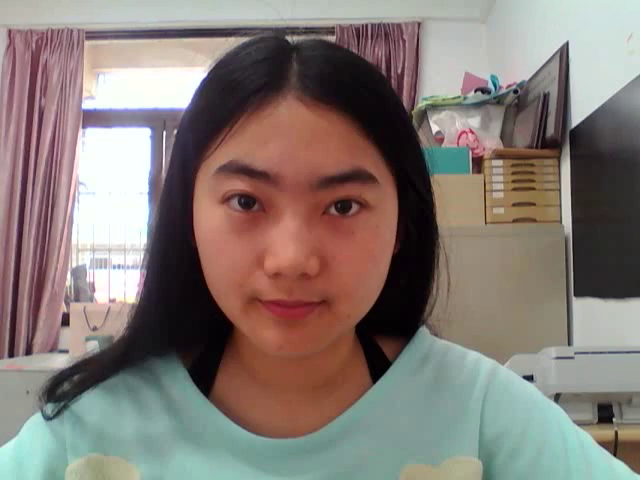
\includegraphics[width=.4\textwidth]{grabcut-original.png}
  }\qquad
  \subfloat[区域跟踪结果]{%
    \label{fig:grabcut-track}
    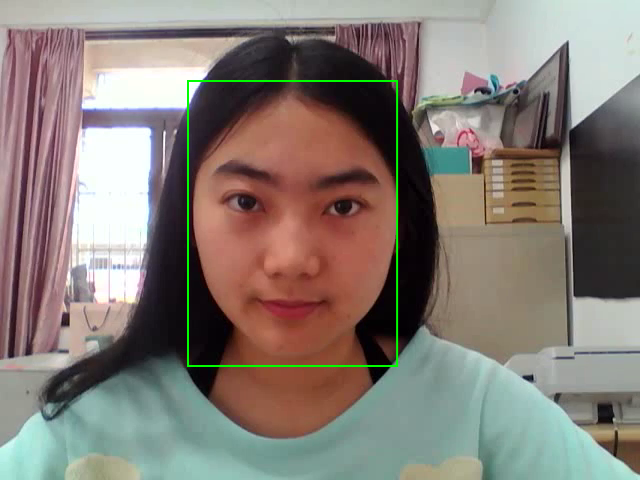
\includegraphics[width=.4\textwidth]{grabcut-track.png}
  }\qquad\\
  \subfloat[使用GrabCut提取得到的前景掩码]{%
    \label{fig:grabcut-mask}
    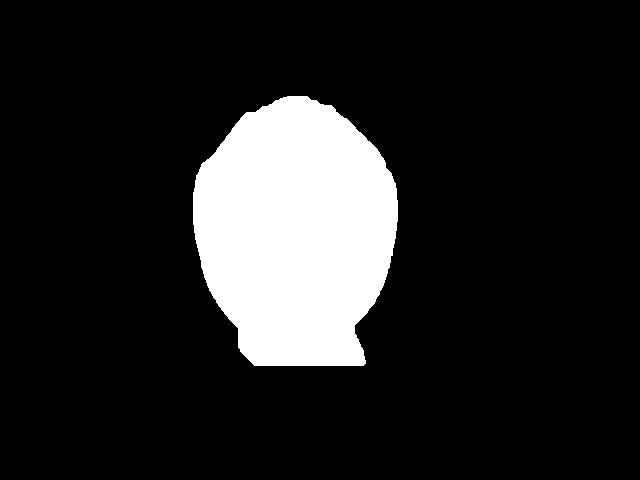
\includegraphics[width=.4\textwidth]{grabcut-mask.png}
  }\qquad
  \subfloat[截取结果]{%
    \label{fig:grabcut-roi}
    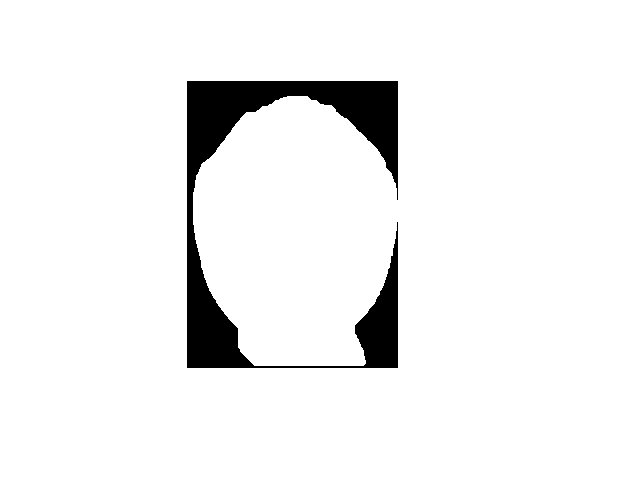
\includegraphics[width=.4\textwidth]{grabcut-roi.png}
  }\qquad
  \caption{使用GrabCut算法从目标区域进一步提取出前景区域}
  \label{fig:grabcut-result}
\end{figure}

\section{局部欧拉影像动作放大}
\label{sec:local-evm}

完成了区域跟踪和前景分割后,接下来对每一帧的目标区域进行欧拉影像动作放大。放大算
法可以使用线性的方法\upcite{wu2012eulerian}或者基于相位的方
法\upcite{Wadhwa2013PhaseBased}。

\subsection{基于CIEL*a*b*空间的颜色衰减}
\label{sec:cielab}

为了抑制噪声,上述两种方法在进行动作放大前,先将视频的每一帧图像由RGB颜色空间转
换为YIQ色彩空间\upcite{buchsbaum1968color}。YIQ是NTSC电视机系统所采用的颜色
空间,其中,Y 是亮度信号,I和Q是色相信号。然后分别对Y、I、Q三个通道的进行时
频处理。之后,引入一个衰减因子$\mu$($0\le \mu \le 1$)衰减I、Q两个通道的变化。
如果要放大动作的变化,可以让$\mu$取一个接近0的值,减少对颜色变化的放大,从而
抑制颜色噪点;如果要放大颜色的变化,则可以让$\mu$取一个接近1的值。

与上述方法不同,本文在进行动作放大前,并不将图像从RGB颜色空间转为YIQ色彩空间,
而是转为更感知均匀的 CIEL*a*b* 颜色空间\upcite{mcguire1992reporting}。其中,L* 分
量密切匹配人类亮度感知,a* 和 b* 分量则分别为红/绿和黄/蓝对立通道。L*、a* 和 b*
的非线性关系可以模仿人眼的非线性响应。图\ref{fig:cielab}是 CIEL*a*b* 颜色空间的
一个彩色模型图。

\begin{figure}[htbp]
  \centering
  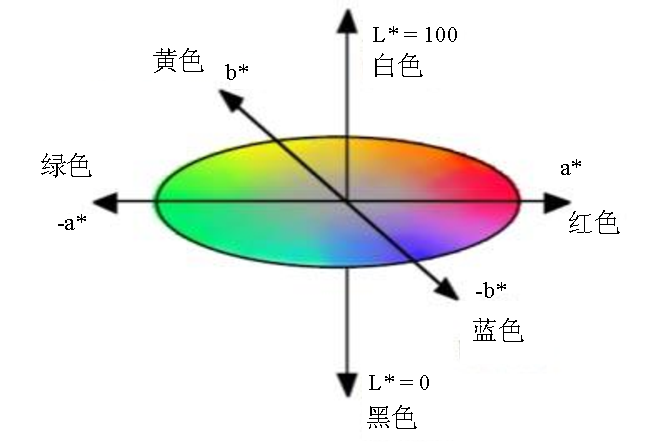
\includegraphics[width=.5\textwidth]{color-plate.pdf}
  \caption{CIEL*a*b*颜色空间模型图}
  \label{fig:cielab}
\end{figure}

要将图像由RGB颜色空间转换到CIEL*a*b*颜色空间,首先先将图像每一个像素的RGB分
量的值归一化为$[0, 1]$之间的浮点数,然后转换到设备无关的XYZ三色值:
\begin{eqnarray*}
  & \begin{bmatrix} X \\ Y \\ Z \end{bmatrix} \leftarrow
  \begin{bmatrix}
    0.412453 & 0.357580 & 0.180423 \\
    0.212671 & 0.715160 & 0.072169 \\
    0.019334 & 0.119193 & 0.950227 \\
  \end{bmatrix}
  \cdot
  \begin{bmatrix}
    R \\ G \\ B
  \end{bmatrix}\\
  & X \leftarrow X/X_n\\
  & Z \leftarrow Z/Z_n
\end{eqnarray*}

其中$X_n = 0.950456$,$Z_n = 1.088754$。

之后将XYZ三色值转为L*、a*、b*的对应值:
\begin{eqnarray*}
  L* & \leftarrow & 116f(Y/Y_n)-16\\
  a* & \leftarrow & 500(f(X/X_n)-f(Y/Y_n))\\
  b* & \leftarrow & 200(f(Y/Y_n)-f(Z/Z_n))
\end{eqnarray*}

其中
\begin{displaymath}
  f(t)=\left\{
    \begin{aligned}
      & t^{1/3} &, t > (\frac{6}{29})^3\\
      & \frac{1}{3}(\frac{29}{6})^2t + \frac{4}{29} &, t \le (\frac{6}{29})^3
    \end{aligned}
\right.
\end{displaymath}

这里的$X_n$,$Y_n$和 $Z_n$是参照白点的CIE XYZ三色值。

将图像由RGB颜色空间转为更加符合人类视觉感知的CIEL*a*b*颜色空间后,对图像进行
动作放大后仍然可以引入衰减因子$\mu$衰减a*、b*两个通道的变化。
图\ref{fig:attenuation}给出了放大face案例的动作后使用$\mu = 0.1$对a*、b*
两个通道的变化进行衰减的结果对比。

\begin{figure}[htbp]
  \centering
  \subfloat[衰减前,图像存在较多颜色噪点]{
    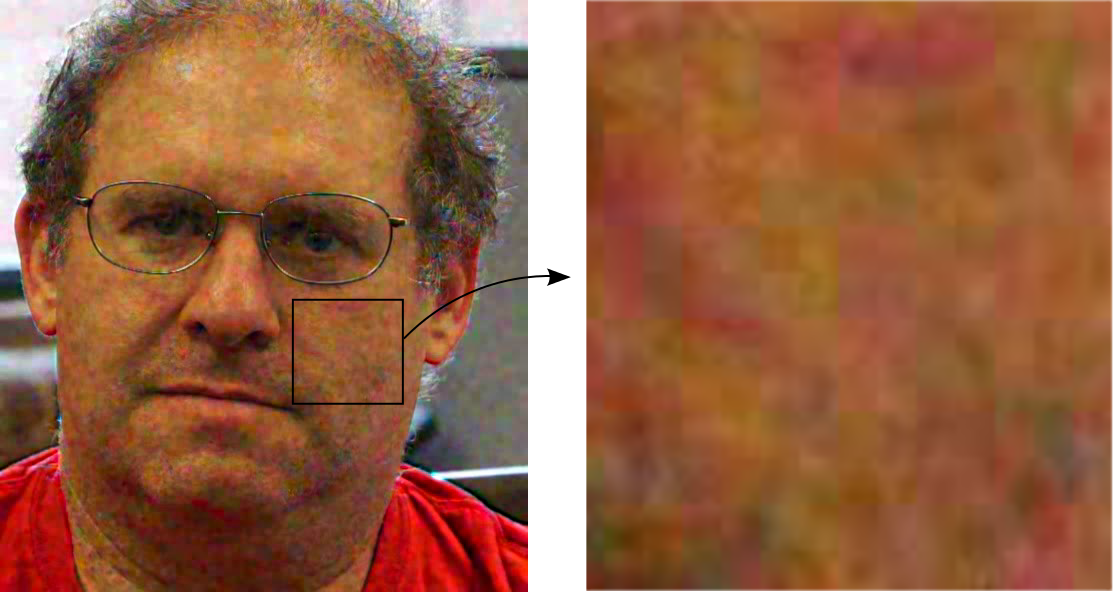
\includegraphics[width=.8\textwidth]{attenuation-before.png}
  }\\
  \subfloat[衰减后,颜色噪点被消除]{
    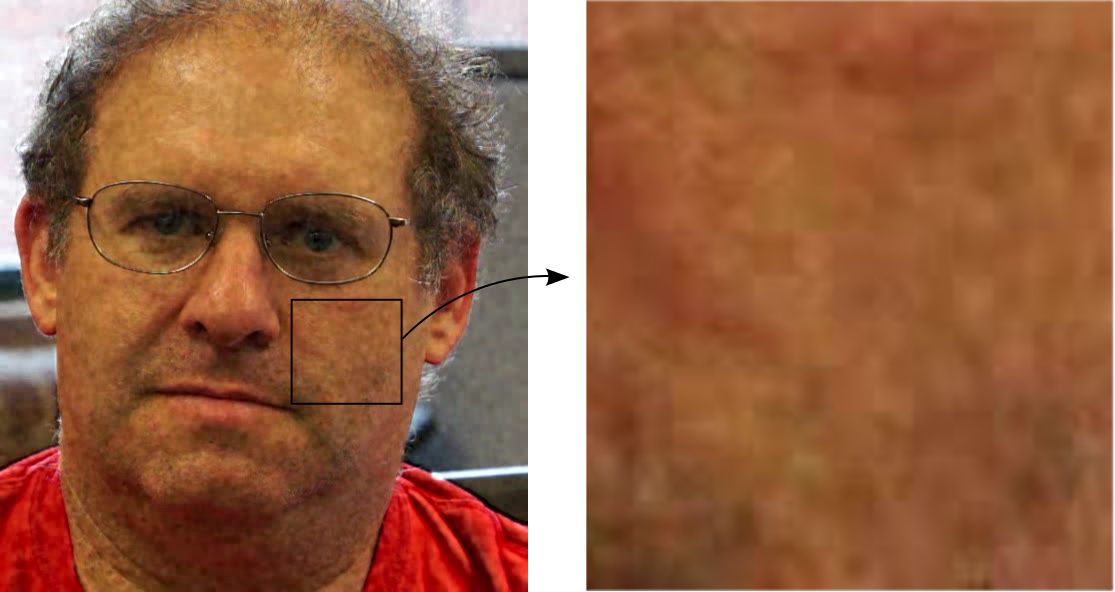
\includegraphics[width=.8\textwidth]{attenuation-after.png}
  }
  \caption{对a*、b*两个通道的变化进行衰减前后结果对比}
  \label{fig:attenuation}
\end{figure}

\subsection{基于四元数的理想带通滤波}
\label{sec:real-quaternion-fourier}

如\ref{sec:eulerian}所述,得到不同空间频率的基带后,对每一基带进行带通滤波,可以
得到感兴趣的变化信号。对于不需要对放大结果进行后续的时频分析的场合,本文使用宽通
带的二阶无限脉冲响应带通滤波器进行带通滤波,该滤波器利用前后帧的差分关系来进行滤
波,因而无需进行时频转换\upcite{storn1996differential};而对于需要对放大结果进行
后续的时频分析的场合,本文使用窄通带的理想带通滤波器进行带通滤波。

对一幅灰度图像进行频率域的理想带通滤波前,需要先对图像进行傅里叶变换,将其转换到
频率域,再构造一个滤波器与之做乘积。二维数字图像的傅里叶变换(DFT)定义为:
\begin{equation}
  \label{eq:dft}
  F(u,v)=\sum_{x=0}^{M-1}\sum_{y=0}^{N-1}f(x,y)e^{-j2\pi(ux/M+vy/N)}
\end{equation}

其中,离散变量$u$,$v$满足$u=0,1,2,\ldots,M-1$,$v=0,1,2,\ldots,N-1$。

由于彩色图像无法直接进行傅里叶变换,因此,文献\cite{wu2012eulerian}及文
献\cite{Wadhwa2013PhaseBased}需要先将每一基带的彩色图像分离成Y、I、Q三个通道图像,
然后对每一个通道的图像单独进行傅里叶变换及带通滤波。

对彩色图像进行理想带通滤波的过程如算
法\ref{alg:temporal-filter}所示\upcite{Gonzalez:2006:DIP:1076432}:

\begin{algorithm}[htbp]
  \caption{理想带通滤波器滤波步骤}
  \label{alg:temporal-filter}
  \begin{algorithmic}[1]
    \REQUIRE 大小为$M\times N$的彩色图像$f(x,y)$。
    \ENSURE 滤波结果$g(x,y)$。
    \STATE 通道分解:将彩色图像$f(x,y)$分成三个通道的图像$f_1(x,y)$,
    $f_2(x,y)$和$f_3(x,y)$。对每幅图像分别执行第2$\sim$7步。
    \STATE 填充图像:对$f_i(x,y)$填充必要数量的0,形成大小为$P\times Q$的填充后的图像
    $f_{p}(x,y)$。其中,$P$和$Q$分别是满足$P\le 2M-1$和$Q\le 2N-1$的最小偶整数。
    \STATE 中心化图像:用$(-1)^{x,y}$乘以$f_{p}(x,y)$,使其移到变换的中心。
    \STATE DFT:根据公式\ref{eq:dft}计算来自步骤3的图像的DFT,得到$F(u,v)$。
    \STATE 理想带通滤波:生成一个实的、对称的理想带通滤波函数 $H(u,v)$,其大小为
    $P\times Q$,中心在$(P/2, Q/2)$处,对图像进行带通滤波操作:$$G(u,v)=H(u,v)F(u,v)$$
    \STATE IDFT:得到处理后的图像:$$g_p(x,y)=\left\{
      \mbox{real}[\Im^{-1}[G(u,v)]] \right\}(-1)^{x+y}$$ 其中,$\Im^{-1}$是IDFT,
    下标$p$用于表明$g_p(x,y)$是填充后的序列。
    \STATE 提取结果:从$g_p(x,y)$的左象限提取$M\times N$区域,得到该通道的滤波结
    果$g_i(x,y)$。
    \STATE 合并通道:将三个单通道的滤波结果$g_1(x,y)$,$g_2(x,y)$和$g_3(x,y)$重新合成一幅彩色图像$g(x,y)$。
  \end{algorithmic}
\end{algorithm}

与上述方法不同,本文在进行理想带通滤波时,并不显式地分离彩色图像的三个通道,而是
将彩色图像的L*、a*、b*三个分量放入一个四元数\upcite{hamilton1866elements}的矢量部
分,形成一个纯四元数。然后直接对其进行傅里叶变换和带通滤波等时频处理,具备更好的整体性。

一个四元数是如下形式的超复数:
\begin{equation}
  \label{eq:quaternion}
  q=a+bi+cj+dk
\end{equation}

其中,$a$、$b$、$c$和$d$是实数,$i$、$j$和$k$是复数单位,且满足:
\begin{equation}
  \label{eq:ijk}
  i^2=j^2=k^2=-1\mbox{,}ij=-ji=k\mbox{,}jk=-kj=i\mbox{,}ik=-ki=-j
\end{equation}

四元数的模定义为:$\left|q\right|=\sqrt{a^2+b^2+c^2+d^2}$,共轭定义为:$\bar{q}=a-bi-cj-dk$。

模为1的四元数称为单位四元数,实部为0的四元数称为纯四元数。

文献\cite{sangwine2000discrete}给出了一般性的四元数傅里叶变换:
\begin{equation}
  \label{eq:quaternion-dft}
  F(u,v)=\frac{1}{\sqrt{MN}}\sum_{y=0}^{M-1}\sum_{x=0}^{N-1}e^{-\mu 2\pi((yv/M)+(xu/N))}f(x,y)
\end{equation}

在本文中,$f$是包含了L*,a*,b*三个分量的二维向量,即
\begin{equation}
  \label{eq:quaternion-lab}
  f(x,y)=L^{*}(x,y)i+a^{*}(x,y)j+b^{*}(x,y)k
\end{equation}

算法\ref{alg:quaternion-temporal-filter}给出了基于四元数的理想带通滤波的步骤。

\begin{algorithm}[htbp]
  \caption{基于四元数的理想带通滤波器滤波步骤}
  \label{alg:quaternion-temporal-filter}
  \begin{algorithmic}[1]
    \REQUIRE 大小为$M\times N$的四元数向量$f(x,y)$。
    \ENSURE 滤波结果 $g(x,y)$。
    \STATE 填充图像:对$f(x,y)$填充必要数量的0,形成大小为$P\times Q$的填充后的图像
    $f_{p}(x,y)$。其中,$P$和$Q$分别是满足$P\le 2M-1$和$Q\le 2N-1$的最小偶整数。
    \STATE 中心化图像:用$(-1)^{x,y}$乘以$f_{p}(x,y)$,使其移到变换的中心。
    \STATE DFT:根据公式\ref{eq:quaternion-dft}计算来自步骤3的图像的DFT,得到$F(u,v)$。
    \STATE 理想带通滤波:生成一个实的、对称的理想带通滤波函数 $H(u,v)$,其大小为
    $P\times Q$,中心在$(P/2, Q/2)$处,对图像进行带通滤波操作:$$G(u,v)=H(u,v)F(u,v)$$
    \STATE IDFT:得到处理后的图像:$$g_p(x,y)=\left\{
      \mbox{real}[\Im^{-1}[G(u,v)]] \right\}(-1)^{x+y}$$ 其中,$\Im^{-1}$是IDFT,
    下标$p$用于表明$g_p(x,y)$是填充后的序列。
    \STATE 提取结果:从$g_p(x,y)$的左象限提取$M\times N$区域,得到该通道的滤波结
    果$g(x,y)$。
  \end{algorithmic}
\end{algorithm}


\section{金字塔混合}
\label{sec:pyramid-blending}

如第\ref{sec:grabcut}节所述,直接对目标区域组成的图像序列进行动作放大会把背景
部分的动作也一同放大。因此,可利用每一帧目标区域对应的前景掩码,将放大结果进一步
约束在前景区域。

最直接的做法是单基带混合:利用前景掩码,从经过放大的动作中取出前景的部分,然后与
原图叠加。但由于动作信号被放大后,部分像素的亮度会增加,此时如果直接与原图叠加,
在目标区域与其他区域间仍然可能出现较生硬的边界。因此,本文采用多基带的金字塔混合
的方法\upcite{ogden1985pyramid},利用前景掩码对目标区域原图和动作放大结果进行金字
塔混合。

考虑图像$A$ 、图像$B$以及掩码图$M$。则对$A$和$B$进行金字塔混合的步骤如算
法\ref{alg:blend}所示。

\begin{algorithm}[htbp]
  \caption{金字塔混合}
  \label{alg:blend}
  \begin{algorithmic}[1]
    \REQUIRE 大小相同的图像$A$,图像$B$及掩码图$M$。
    \ENSURE 混合结果$C$。
    \STATE 分别由图像$A$和图像$B$构造$n$层拉普拉斯金字塔$P_A$和$P_B$,
    由图像$M$构造$n$层高斯金字塔$P_M$。
    \STATE 对每一层基带,单独进行上述的单基带混合,将混合结果存入一个新的拉普拉
    斯金字塔$P_C$的相同层。
    \STATE 根据$P_C$重建出图像$C$ 。
  \end{algorithmic}
\end{algorithm}

在本文中,$P_A$、$P_B$分别是经放大后的动作信息和原图的拉普拉斯金字塔,而$P_M$则
为前景掩码的高斯金字塔,这三个图像金字塔在进行欧拉影像动作放大时已经构造完成,因
此无需再执行算法\ref{alg:blend}中的第1步。

图\ref{fig:blend-compare}给出了单基带混合和金字塔混合的结果对比。经过单基带混合
后,女孩的脖子处依然存在明显的边界。而经过金字塔混合后,脖子处的边界已经被消除。

\clearpage

\begin{figure}[htbp]
  \centering
  \subfloat[单基带混合,仍然可能存在边界]{
    \label{fig:single-band}
  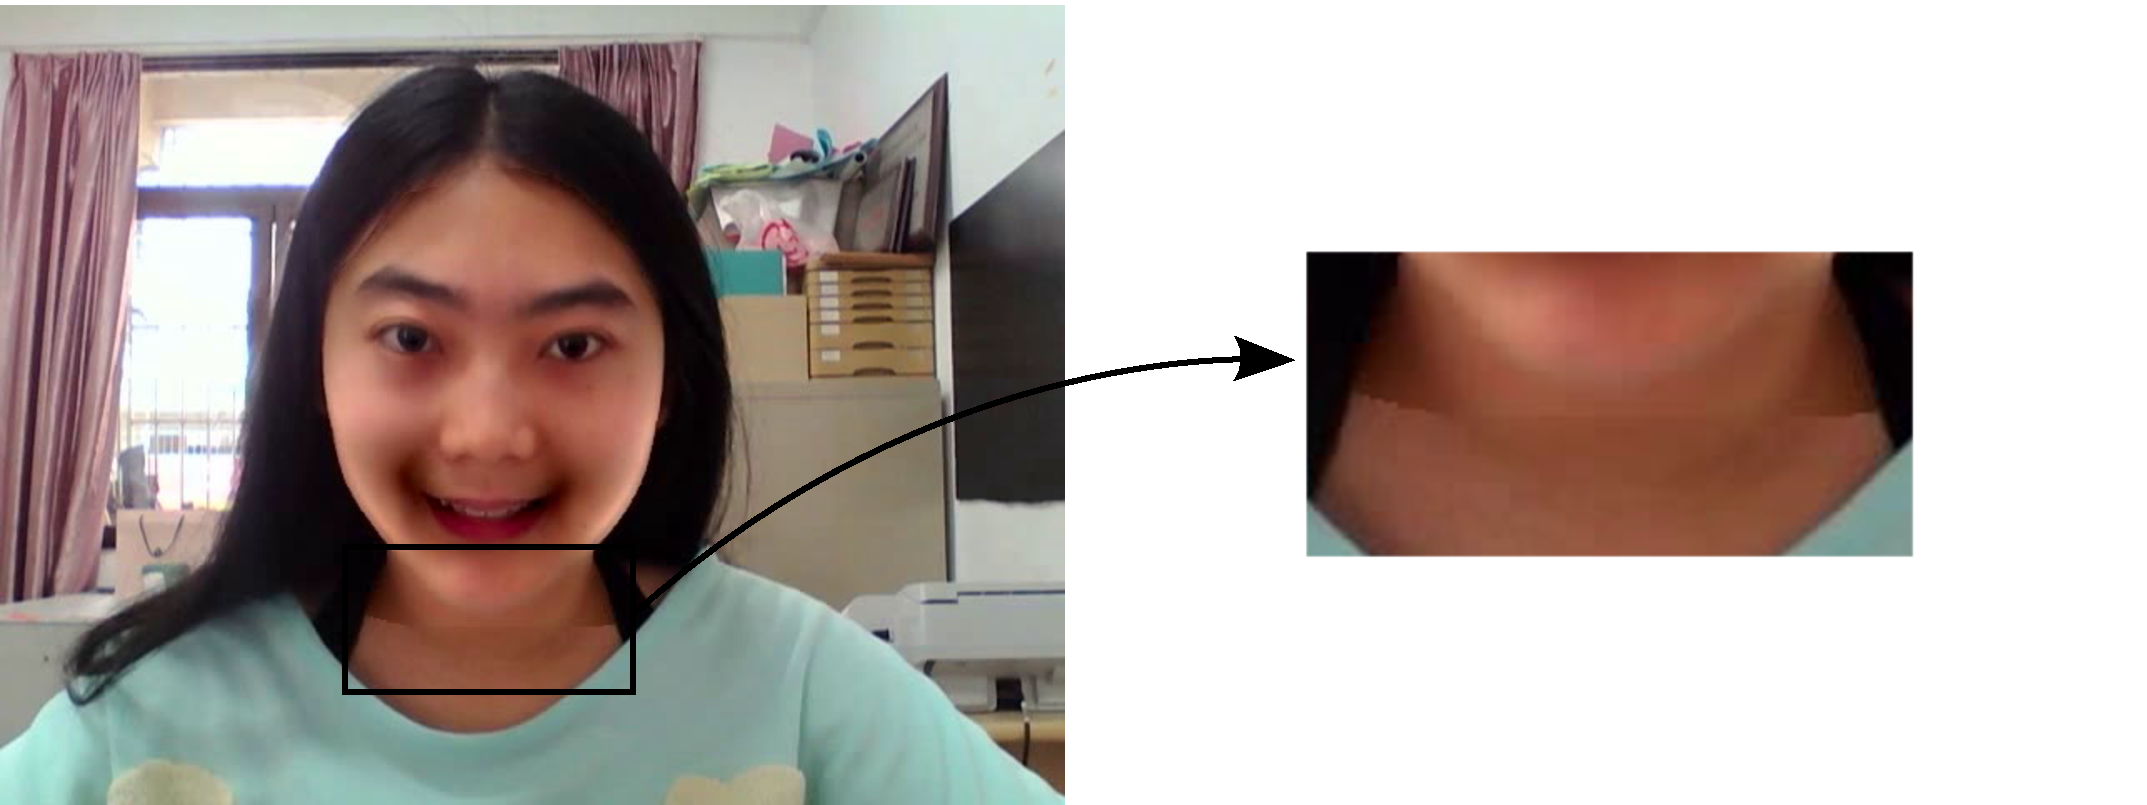
\includegraphics[width=.8\textwidth]{single-band-blend-asy.pdf}
  }\\
  \subfloat[金字塔混合,边界问题得到改善]{
    \label{fig:multi-band}
    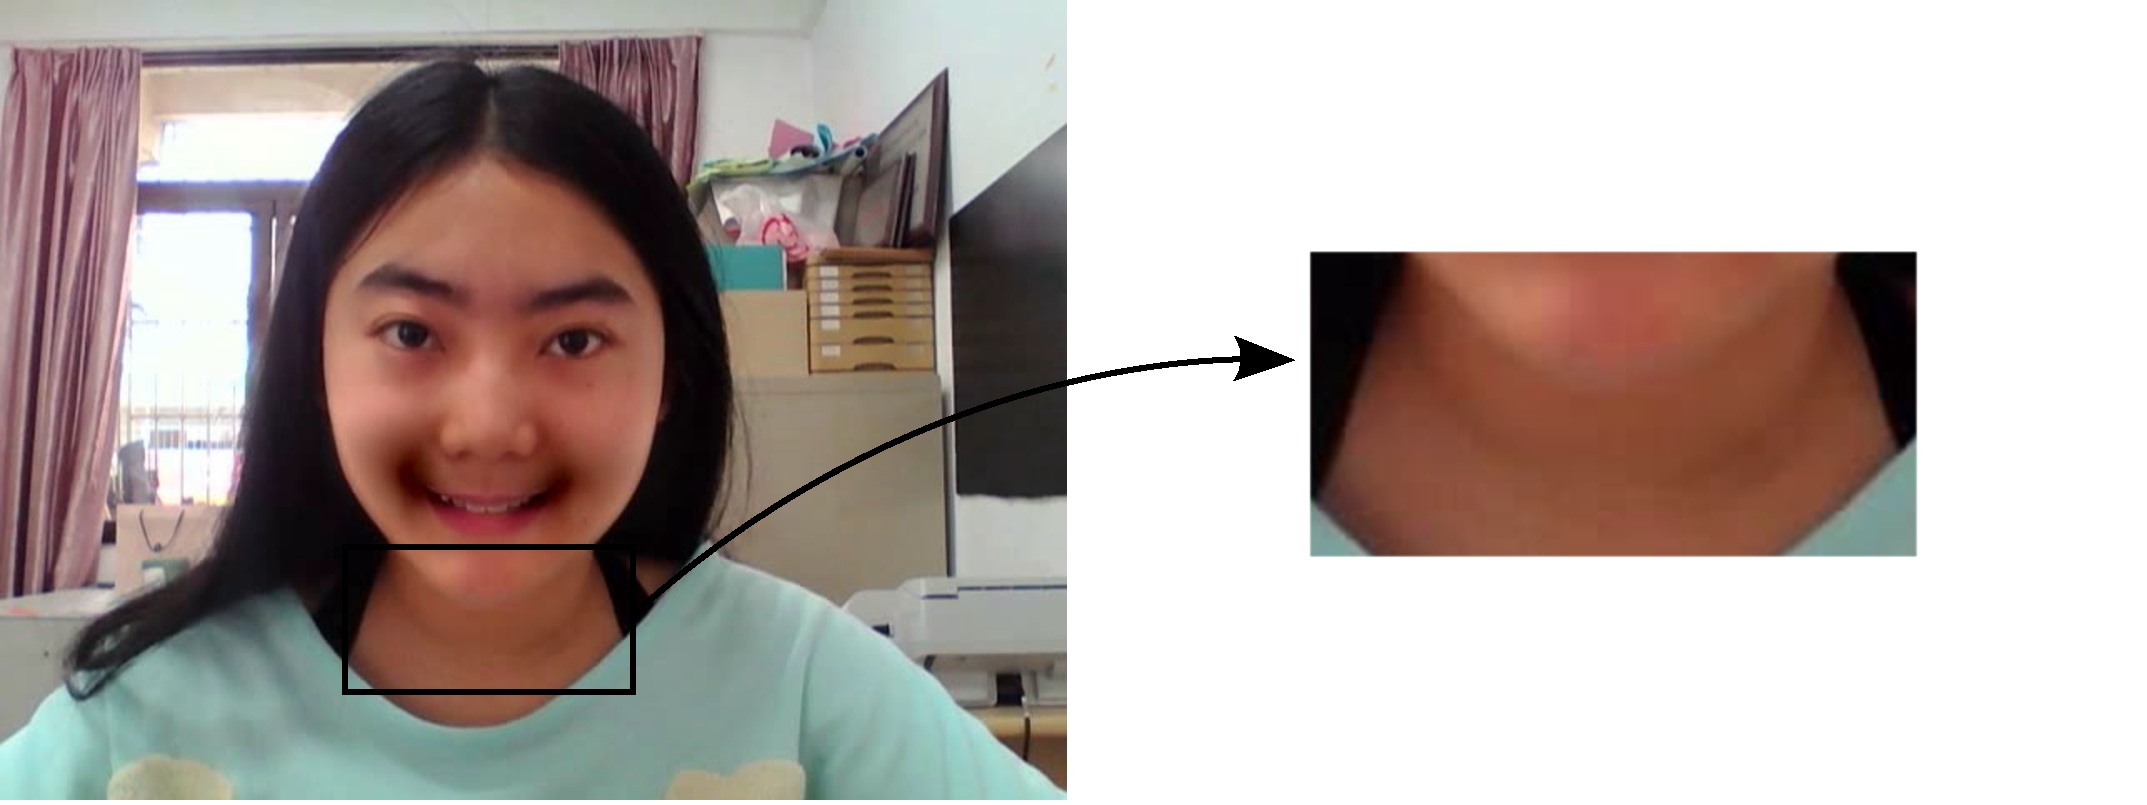
\includegraphics[width=.8\textwidth]{pyramid-blend-asy.pdf}
  }
  \caption{单基带混合和金字塔混合的结果对比}
  \label{fig:blend-compare}
\end{figure}

%%% Local Variables: 
%%% mode: latex
%%% TeX-master: "../thesis"
%%% End: 


\chapter{教程}

\section{字体段落}
\label{sec:font}

本节内容来自华南师范大学外部门户\footnote{外部门户主页:\url{http://www.scnu.edu.cn/}}。

华南师范大学始建于1933年,是一所学科门类齐全的国家“211 工程”重点建设大学和广东%
省省属重点大学。学校现有广州石牌、广州大学城和南海3个校区,占地面积共3079亩,%
校舍面积共 126万平方米。校园环境优美,景色怡人~,人文景观遍布,文化气息浓厚,为广%
大师生提供了良好的学习、工作和生活环境。

学校现有4个国家重点学科(含1个重点培育学科), 9个国家“211 工程”重点建设学%
科,2个广东省一级学科重点学科,11个广东省二级学科重点学科。有71个本科专业,有14个%
博士学位授权一级学科、90个博士学位授权点(未含2011年8月一级学科调整后新增的博士%
点)、1个博士专业学位授权点,33个硕士学位授权一级学科、174个硕士学位授权点(未%
含2011年8月一级学科调整后新增的硕士点)、10个硕士专业学位授权点,涉及到哲学、经济%
学、法学、教育学、文学、历史学、理学、工学、管理学、农学、医学等11个学科门%
类。 有12个博士后流动站。

学校拥有一批实力较强的实验室和科研基地。有教育部激光生命科学重点实验室、环境理论
化学重点实验室(省部共建)、教育部电化学储能材料与技术工程研究中心、卫生部(中医
药管理局)中医药与光子技术实验室、国家理科基础科学研究和教学人才培养基地、教育部
部省共建人文社科重点研究基地(心理应用研究中心)、国家体育总局重点研究基地(体育
社会科学研究基地),有7个广东省重点实验室(中心),6个广东省高校科研型重点实验
室,3个广东省高校产学研结合示范基地,6个广东省普通高校人文社会科学重点研究基
地,1个广东省高校工程技术研究中心。学校还拥有“物理学科基础课”、“信息传
播”~、“心理学”等3个国家级实验教学示范中心,7个广东省实验教学示范中心。此外,教
育部高校辅导员培训和研修基地、广东省普通高等学校师资培训中心~、广东省网络图书馆、
广东高校建筑规划设计院等机构均设在学校。

70 多年来,学校数易校名,几度迁徙,虽历经沧桑,却弦歌不辍。一代又一代华师人秉承勷
勤大学师范学院{\kai “研究高深学术,养成社会之专门人才”}的优良传统,承传南方大
学{\kai “忠诚团结,朴实虚心,勤劳勇敢,实事求是”}的革命精神~,践行{\kai “艰苦奋斗、严谨治
学、求实创新、为人师表”}的校训,筚路蓝缕,薪火相传,共同铸就了学校今天的繁荣与
发展。

华南师范大学历史上的名字包括:

\begin{itemize}
\item[楷体] {\kai 广州市立师范学校}
\item[黑体] {\hei 勷勤大学师范学院}
\item[隶书] {\li 勷勤大学教育学院}
\item[宋体] {\song 广东省立教育学院}
\item[仿宋] {\fs 广东省立文理学院}
\item[粗体] {\bfseries 广东省文理学院}
\item[斜体] {\itshape 华南师范学院}
\item[粗斜体] {\bfseries\itshape 广东师范学院}
\item[字体颜色] {\textcolor{red}{华南师范大学}}
\end{itemize}

上面这段内容使用了itemize列表环境,\LaTeX{}默认的列表环境会在条目之间插入
过多的行距,若用户需要紧凑的行距,可以使用compactitem环境。

下面测试英文字体:

Remember the \textsf{more} \textbf{font} {\bfseries\tiny you \sffamily use,
\Large the \scshape more \itshape beautiful \slshape your \footnotesize
document becomes.}

\begin{itemize}
\item[英文黑体] Typeset text in \textbf{bold} series
\item[英文斜体] Typeset text in \textit{italic} shape
\item[Roman字体] Typeset text in roman family
\item[Sans Serif字体] Typeset text in \textsf{sans serif} family
\item[typewriter字体] Typeset text in \texttt{typewriter} family
\end{itemize}

下面测试字号:
\begin{itemize}
\item[初号] {\chuhao 华南师范大学}
\item[小初] {\xiaochu 华南师范大学}
\item[一号] {\yihao 华南师范大学}
\item[小一] {\xiaoyi 华南师范大学}
\item[二号] {\erhao 华南师范大学}
\item[小二] {\xiaoer 华南师范大学}
\item[三号] {\sanhao 华南师范大学}
\item[小三] {\xiaosan 华南师范大学}
\item[四号] {\sihao 华南师范大学}
\item[小四] {\xiaosi 华南师范大学}
\item[五号] {\wuhao 华南师范大学}
\item[小五] {\xiaowu 华南师范大学}
\end{itemize}

\section{表格明细}
\label{sec:figure}
表格是书中的重要组成部分,这一章将从简单的表格讲起,到复杂的表格为止。

\subsection{基本表格}
\label{sec:basictable}

模板中关于表格的宏包有三个: \textsf{booktabs}、\textsf{array} 和
\textsf{longtabular},命令有一个 \verb|\hlinewd|。三线表建议使用\textsf{booktabs}中提供的,
包含toprule、midrule 和 bottomrule三条命令。
它们与\textsf{longtable} 能很好的配合使用。如果表格比较简单的话可以直接用命令
\verb|hlinewd{xpt}| 控制。下面来看一个表格:
\begin{table}[htb]
  \centering
  \begin{minipage}[t]{0.8\linewidth} % 如果想在表格中使用脚注,minipage是个不错的办法
  \caption[模板文件]{模板文件。如果表格的标题很长,那么在表格索引中就会很不美
    观,所以要像 chapter 那样在前面用中括号写一个简短的标题。这个标题会出现在索
    引中。}
  \label{tab:template-files}
    \begin{tabular*}{\linewidth}{lp{10cm}}
      \toprule[1.5pt]
      {\hei 文件名} & {\hei 描述} \\
      \midrule[1pt]
      scnuthesis.ins & \LaTeX{} 安装文件,docstrip\footnote{表格中的脚注} \\
      scnuthesis.dtx & 所有的一切都在这里面\footnote{再来一个}。\\
      scnuthesis.cls & 模板类文件。\\
      scnuthesis.cfg & 模板配置文。cls 和 cfg 由前两个文件生成。\\
      bstutf8.bst   & 参考文献 Bibtex 样式文件。\\
      myscnu.sty    & 常用的包和命令写在这里,减轻主文件的负担。\\
      \bottomrule[1.5pt]
    \end{tabular*}
  \end{minipage}
\end{table}

如果你不需要在表格中插入脚注,可以将minipage环境去掉。

表 \ref{tab:template-files} 列举了本模板主要文件及其功能。
请大家注意三线表中各条线对应的命令。这个例子还展示了如何在表格中正确使用脚注。
由于 \LaTeX{} 本身不支持在表格中使用 \verb|\footnote|,所以我们不得不将表格放在
小页中,而且最好将表格的宽度设置为小页的宽度,这样脚注看起来才更美观。

如果遇到表格内容自动调整的问题,可以有两种解决办法: 其一就是用\verb|tabular*|,在
两列之间全部插入空白,该方法存在的缺点是当只有两列需要自动调整时,若小页预留空间
过大,可能插入过多的\verb|fill|,导致不美观; 另外一种就是使用\verb|tabularx|自动
调整了,需要定制一个\textbf{Z}环境,在新版本中,该命令已添加到\verb|myscnu.sty|中。
下面是这两个方法实现的对比,各位可以仔细对比一下,推荐使用后者。

\begin{table}[htbp]
\centering
\begin{minipage}[t]{0.9\linewidth}
\caption{Reed Solomon码的典型应用}
\label{tab:RSused}
\begin{tabular*}{\linewidth}{c @{\extracolsep{\fill}} c}
\toprule[1.5pt]
{\hei 应用领域} & {\hei 编码方案}\\
\midrule[1pt]
磁盘驱动器 & RS(32,28,5)码 \footnote{码长为32、维数为28、最小距离为5} \\
CD & 交叉交织RS码(CIRC) \\
DVD & RS(208,192,17)码、RS(182,172,11)码 \\
光纤通信 & RS(255,229,17)码 \\
\bottomrule[1.5pt]
\end{tabular*}
\end{minipage}
\end{table}

\begin{table}[htbp]
\centering
\begin{minipage}[t]{0.9\linewidth}
\caption{Reed Solomon码的典型应用}
\label{tab:RSuse}
\begin{tabularx}{\linewidth}{cZ}
\toprule[1.5pt]
{\hei 应用领域} & {\hei 编码方案}\\
\midrule[1pt]
磁盘驱动器 & RS(32,28,5)码 \footnote{码长为32、维数为28、最小距离为5} \\
CD & 交叉交织RS码(CIRC) \\
DVD & RS(208,192,17)码、RS(182,172,11)码 \\
光纤通信 & RS(255,229,17)码 \\
\bottomrule[1.5pt]
\end{tabularx}
\end{minipage}
\end{table}

\subsection{复杂表格}
\label{sec:complicatedtable}

我们经常会在表格下方标注数据来源,或者对表格里面的条目进行解释。前面的脚注是一种
不错的方法,如果你不喜欢脚注。那么完全可以在表格后面自己写注释,比如表~\ref{tab:tabexamp1}。
\begin{table}[htbp]
  \centering
  \caption{复杂表格示例 1}
  \label{tab:tabexamp1}
  \begin{minipage}[t]{0.8\textwidth} 
    \begin{tabularx}{\linewidth}{|l|X|X|X|X|}
      \hline
      \multirow{2}*{\backslashbox{x}{y}}  & \multicolumn{2}{c|}{First Half} & \multicolumn{2}{c|}{Second Half}\\
      \cline{2-5}
      & 1st Qtr &2nd Qtr&3rd Qtr&4th Qtr \\ 
      \hline
      East$^{*}$ &   20.4&   27.4&   90&     20.4 \\
      West$^{**}$ &   30.6 &   38.6 &   34.6 &  31.6 \\ 
      \hline
    \end{tabularx}\\[2pt]
    \footnotesize
    *:东部\\
    **:西部
  \end{minipage}
\end{table}

此外,表~\ref{tab:tabexamp1} 同时还演示了另外两个功能:1)通过 \textsf{tabularx} 的
 \texttt{|X|} 扩展实现表格自动放大;2)通过命令 \verb|\backslashbox| 在表头部分
插入反斜线。

为了使我们的例子更接近实际情况,我会在必要的时候插入一些“无关”文字,以免太多图
表同时出现,导致排版效果不太理想。

学校七十余载薪火相传,名师荟萃,著名的教育家罗浚、汪德亮,五四新诗开创者之一康白
情,古代文学家李镜池,古汉语学家吴三立,历史学家王越,逻辑学家李匡武,心理学家阮
镜清,教育学家叶佩华、朱勃,数学家叶述武,物理学家黄友谋、刘颂豪,著名体育教育家
袁浚等众多名家、名师先后在此执教。该校虽数度易名、几经迁徙,但一代又一代华师人秉
承勷勤大学师范学院``研究高深学术,养成社会之专门人才''的优良传统,承传南方大
学``忠诚团结,实事求是''的革命精神,践行``艰苦奋斗、严谨治学、求实创新、为人师
表''的校训,不断推动学校事业向前发展。特别是改革开放以来,抓住科教兴国、人才强国
的发展机遇,凭借建设文化省、教育强省和国家``211工程''的强劲东风,形成了学校现在
跨越式发展的大好局面。

不可否认 \LaTeX{} 的表格功能没有想象中的那么强大,不过只要你足够认真,足够细致,那么
同样可以排出来非常复杂非常漂亮的表格。请参看表~\ref{tab:tabexamp2}。
\begin{table}[htbp]
  \centering\dawu[1.3]
  \caption{复杂表格示例 2}
  \label{tab:tabexamp2}
  \begin{tabular}[c]{|c|m{0.8in}|c|c|c|c|c|}\hline
    \multicolumn{2}{|c|}{Network Topology} & \# of nodes & 
    \multicolumn{3}{c|}{\# of clients} & Server \\\hline
    GT-ITM & Waxman Transit-Stub & 600 &
    \multirow{2}{2em}{2\%}& 
    \multirow{2}{2em}{10\%}& 
    \multirow{2}{2em}{50\%}& 
    \multirow{2}{1.2in}{Max. Connectivity}\\\cline{1-3}
    \multicolumn{2}{|c|}{Inet-2.1} & 6000 & & & &\\\hline
    \multirow{2}{1in}{Xue} & Rui  & Ni &\multicolumn{4}{c|}{\multirow{2}*{\scnuthesis}}\\\cline{2-3}
    & \multicolumn{2}{c|}{ABCDEF} &\multicolumn{4}{c|}{} \\\hline
\end{tabular}
\end{table}

\subsection{子表格与跨页表格}

浮动体的并排放置一般有两种情况:1)二者没有关系,为两个独立的浮动体;2)二者隶属
于同一个浮动体。对表格来说并排表格既可以像图~\ref{tab:parallel1}、图~\ref{tab:parallel2} 
使用小页环境,也可以如图~\ref{tab:subtable} 使用子表格来做。后面我们将讲解图的例子。
\begin{table}[htb]
\noindent\begin{minipage}{0.45\textwidth}
\centering
\caption{第一个并排子表格}
\label{tab:parallel1}
\begin{tabular}{p{2cm}p{2cm}}
\toprule[1.5pt]
111 & 222 \\\midrule[1pt]
222 & 333 \\\bottomrule[1.5pt]
\end{tabular}
\end{minipage}
\begin{minipage}{0.45\textwidth}
\centering
\caption{第二个并排子表格}
\label{tab:parallel2}
\begin{tabular}{p{2cm}p{2cm}}
\toprule[1.5pt]
111 & 222 \\\midrule[1pt]
222 & 333 \\\bottomrule[1.5pt]
\end{tabular}
\end{minipage}
\end{table}

学校教师队伍结构良好、水平较高,拥有一批在国内外具有一定影响的专家学者。现有教师
队伍 1900 多人,其中教授 400 多人,副教授 500 多人,博士、硕士研究生导师 800 多人,
具有博士、硕士学位和研究生学历的1500 多人。在师资队伍中,有中国科学院院士 7 人、
瑞典皇家科学院院士2人、“千人计划”入围者 1人、长江学者4人、获得国家杰出青年基金
项目资助者3人、“新世纪百千万人才”国家级人选 5人、国家级教学名师2 人、广东省领军
人才4人、珠江学者4人、广东省高等学校“千百十工程”国家级培养对象5人,拥有教育
部“长江学者与创新团队发展计划”创新团队 1个、广东省创新科研团队1个,并有国务院学
位委员会学科评议组成员 3 人、教育部高等学校教学指导委员会成员 12 人。

\begin{table}[htbp]
\centering
\caption{并排子表格}
\label{tab:subtable}
\subfloat[第一个子表格]{
\begin{tabular}{p{2cm}p{2cm}}
\toprule[1.5pt]
111 & 222 \\\midrule[1pt]
222 & 333 \\\bottomrule[1.5pt]
\end{tabular}}\hskip2cm
\subfloat[第二个子表格]{
\begin{tabular}{p{2cm}p{2cm}}
\toprule[1.5pt]
111 & 222 \\\midrule[1pt]
222 & 333 \\\bottomrule[1.5pt]
\end{tabular}}
\end{table}

如果您要排版的表格长度超过一页,那么推荐使用 \textsf{longtable} 或者 \textsf{supertabular} 
宏包,表~\ref{tab:performance} 就是 \textsf{longtable} 的简单示例。
\begin{longtable}[c]{c*{6}{r}}
\caption{实验数据}\label{tab:performance}\\
\toprule[1.5pt]
 测试程序 & \multicolumn{1}{c}{正常运行} & \multicolumn{1}{c}{同步}
& \multicolumn{1}{c}{检查点}   & \multicolumn{1}{c}{卷回恢复}
& \multicolumn{1}{c}{进程迁移} & \multicolumn{1}{c}{检查点} 	\\
& \multicolumn{1}{c}{时间 (s)} & \multicolumn{1}{c}{时间 (s)}
& \multicolumn{1}{c}{时间 (s)} & \multicolumn{1}{c}{时间 (s)}
& \multicolumn{1}{c}{时间 (s)} &  文件(KB)			\\
\midrule[1pt]%
\endfirsthead%

\multicolumn{7}{c}{续表~\thetable\hskip1em 实验数据}\\

\toprule[1.5pt]
 测试程序 & \multicolumn{1}{c}{正常运行} & \multicolumn{1}{c}{同步} 
& \multicolumn{1}{c}{检查点}   & \multicolumn{1}{c}{卷回恢复}
& \multicolumn{1}{c}{进程迁移} & \multicolumn{1}{c}{检查点} 	\\
& \multicolumn{1}{c}{时间 (s)} & \multicolumn{1}{c}{时间 (s)}
& \multicolumn{1}{c}{时间 (s)} & \multicolumn{1}{c}{时间 (s)}
& \multicolumn{1}{c}{时间 (s)} &  文件(KB)			\\
\midrule[1pt]%
\endhead%
\hline%

\multicolumn{7}{r}{续下页}%

\endfoot%
\endlastfoot%
CG.A.2 & 23.05   & 0.002 & 0.116 & 0.035 & 0.589 & 32491  \\
CG.A.4 & 15.06   & 0.003 & 0.067 & 0.021 & 0.351 & 18211  \\
CG.A.8 & 13.38   & 0.004 & 0.072 & 0.023 & 0.210 & 9890   \\
CG.B.2 & 867.45  & 0.002 & 0.864 & 0.232 & 3.256 & 228562 \\
CG.B.4 & 501.61  & 0.003 & 0.438 & 0.136 & 2.075 & 123862 \\
CG.B.8 & 384.65  & 0.004 & 0.457 & 0.108 & 1.235 & 63777  \\
MG.A.2 & 112.27  & 0.002 & 0.846 & 0.237 & 3.930 & 236473 \\
MG.A.4 & 59.84   & 0.003 & 0.442 & 0.128 & 2.070 & 123875 \\
MG.A.8 & 31.38   & 0.003 & 0.476 & 0.114 & 1.041 & 60627  \\
MG.B.2 & 526.28  & 0.002 & 0.821 & 0.238 & 4.176 & 236635 \\
MG.B.4 & 280.11  & 0.003 & 0.432 & 0.130 & 1.706 & 123793 \\
MG.B.8 & 148.29  & 0.003 & 0.442 & 0.116 & 0.893 & 60600  \\
LU.A.2 & 2116.54 & 0.002 & 0.110 & 0.030 & 0.532 & 28754  \\
LU.A.4 & 1102.50 & 0.002 & 0.069 & 0.017 & 0.255 & 14915  \\
LU.A.8 & 574.47  & 0.003 & 0.067 & 0.016 & 0.192 & 8655   \\
LU.B.2 & 9712.87 & 0.002 & 0.357 & 0.104 & 1.734 & 101975 \\
LU.B.4 & 4757.80 & 0.003 & 0.190 & 0.056 & 0.808 & 53522  \\
LU.B.8 & 2444.05 & 0.004 & 0.222 & 0.057 & 0.548 & 30134  \\
EP.A.2 & 123.81  & 0.002 & 0.010 & 0.003 & 0.074 & 1834   \\
EP.A.4 & 61.92   & 0.003 & 0.011 & 0.004 & 0.073 & 1743   \\
EP.A.8 & 31.06   & 0.004 & 0.017 & 0.005 & 0.073 & 1661   \\
EP.B.2 & 495.49  & 0.001 & 0.009 & 0.003 & 0.196 & 2011   \\
EP.B.4 & 247.69  & 0.002 & 0.012 & 0.004 & 0.122 & 1663   \\
EP.B.8 & 126.74  & 0.003 & 0.017 & 0.005 & 0.083 & 1656   \\
\bottomrule[1.5pt]
\end{longtable}

为了排版方便,这里要插入一些随机的文字,那就加上猩猩博客的东西吧: 
``越来越喜欢吃,自己做的川菜,每次做菜,都像是创作的过程,%
随心所欲; 发现家常菜真的很难做好,越是简单的菜,越是难以做好。
献上一个鱼香肉丝,让我跟随简单的脚步,creat出简约的菜品。''

\subsection{其它}
\label{sec:tableother}
有的同学不想让某个表格或者图片出现在索引里面,那么请使用命令 \verb|\caption*{}|,
这个命令不会给表格编号,也就是出来的只有标题文字而没有“表~XX”,“图~XX”,否则
索引里面序号不连续就显得不伦不类,这也是 \LaTeX{} 里星号命令默认的规则。

\section{绘图插图}

绘图工具分为 GUI 的和 CLI 两种。GUI即是所见即所得的绘图工具~,常见的包
括 Visio、Inkscape、CorelDraw、XFig(jFig)、WinFig、Tpx、Ipe、Dia等;CLI则是需要编
译后才能够得到图形的工具,比较流行的有 PGF/TikZ~、Asymptote、pstricks等。GUI 类绘
图工具比较易于上手,而 CLI 类绘图工具则能够画出更加精确的图形。关于各类绘图工具的
比较和使用方法~,推荐用户到C\TeX{}论坛{\url{http://bbs.ctex.org/}}以及China\TeX{}论坛
{\url{http://bbs.chinatex.org/forum.php}}上的相关板块进行更加深入的了解。

\subsection{插图}
\label{sec:graphs}

强烈推荐《\LaTeXe 插图指南》!关于子图形使用细节请参看\textsf{subfig}手册。 

\subsubsection{一个图形}
\label{sec:onefig}
一般图形都是处在浮动环境中。之所以称为浮动是指最终排版效果图形的位置不一定与源文
件中的位置对应,这也是刚使
用 \LaTeX{} 同学可能遇到的问题。如果要强制固定浮动图形的位置,请使用 \textsf{float} 宏包,
它提供了 \texttt{[H]} 参数,但是除非特别需要,不建议使用\texttt{[H]},
而是倾向于使用\texttt{[htbp]},给\LaTeX{}更多选择。比如图~\ref{fig:ipe}。
\begin{figure}[htbp] % use float package if you want it here
  \centering
  \includegraphics[width=\textwidth]{tikz}
  \caption{利用TikZ制图}
  \label{fig:ipe}
\end{figure}

大学之道,在明明德,在亲民,在止于至善。知止而后有定;定而后能静;静而后能安;安
而后能虑;虑而后能得。物有本末,事有终始。知所先后,则近道矣。古之欲明明德于天
下者,先治其国;欲治其国者,先齐其家;欲齐其家者~,先修其身;欲修其身者,先正其心;
欲正其心者,先诚其意;欲诚其意者~,先致其知;致知在格物。物格而后知至;知至而后
意诚;意诚而后心正;心正而后身修;身修而后家齐;家齐而后国治;国治而后天下
平。自天子以至于庶人,壹是皆以修身为本。其本乱而未治者 否矣。其所厚者薄,而其所
薄者厚,未之有也!

\hfill \pozhehao《大学》

\subsubsection{多个图形}
\label{sec:multifig}

如果多个图形相互独立,并不共用一个图形计数器,那么用 \verb|minipage| 或者
\verb|parbox| 就可以。否则,请参看图~\ref{fig:big1},它包含两个小图,分别是图~\ref{fig:subfig1} 
和图~\ref{fig:subfig2}。推荐使用 \verb|\subfloat|,不要再用
\verb|\subfigure| 和 \verb|\subtable|。
\begin{figure}[htb]
  \centering%
  \subfloat[第一个小图形]{%
    \label{fig:subfig1}
    \includegraphics[height=2cm]{logo.jpg}}\hspace{4em}%
  \subfloat[第二个小图形。如果标题很长的话,它会自动换行,这个 caption 就是这样的例子]{%
    \label{fig:subfig2}
    \includegraphics[height=2cm]{don-hires}}
  \caption{包含子图形的大图形}
  \label{fig:big1}
\end{figure}

培育英才万万千,建设祖国锦绣河山,华师儿女奋勇当先,珠江滚滚红绵艳~,岭南大地草木
春,改革开放阳光好,华师园里花烂漫。

艰苦奋斗众志坚,严谨治学成风范,求实创新勇开拓,为人师表代代相传,教育改革宏图展,
师范园地好摇篮,培育祖国栋梁材,神圣职责我承担。


下面这个例子显示并排$3\times2$的图片,见图\ref{fig:subfig:3x2}:
\begin{figure}[htb]
\centering
\subfloat[]{\includegraphics[width=.27\textwidth]{typography}} \qquad
\subfloat[]{\includegraphics[width=.27\textwidth]{typography}} \qquad
\subfloat[]{\includegraphics[width=.27\textwidth]{typography}} \qquad
\subfloat[]{\includegraphics[width=.27\textwidth]{typography}} \qquad
\subfloat[]{\includegraphics[width=.27\textwidth]{typography}} \qquad
\subfloat[]{\includegraphics[width=.27\textwidth]{typography}}
\caption{并排图片}
\label{fig:subfig:3x2}
\end{figure}

要注意,\texttt{qquad}相当于\verb|\hspace{2em}|,也就是2个字符的宽度,约0.08倍页宽,
图片宽度设定为0.27倍页宽是合适的;在该环境中,尽量不要手动换行。

向前向前向前向前,华师儿女永远向前!

如果要把编号的两个图形并排,那么小页就非常有用了:
\begin{figure}[htb]
\begin{minipage}{0.48\textwidth}
  \centering
  \includegraphics[height=4cm]{cat.jpg}
  \caption{并排第一个图}
  \label{fig:parallel1}
\end{minipage}\hfill
\begin{minipage}{0.48\textwidth}
  \centering
  \includegraphics[height=4cm]{cat.jpg}
  \caption{并排第二个图}
  \label{fig:parallel2}
\end{minipage}
\end{figure}

\section{公式定理}
\label{sec:equation}
贝叶斯公式如式~(\ref{equ:chap1:bayes}),其中 $p(y|\mathbf{x})$ 为后验;
$p(\mathbf{x})$ 为先验;分母 $p(\mathbf{x})$ 为归一化因子。
\begin{equation}
\label{equ:chap1:bayes}
p(y|\mathbf{x}) = \frac{p(\mathbf{x},y)}{p(\mathbf{x})}=
\frac{p(\mathbf{x}|y)p(y)}{p(\mathbf{x})} 
\end{equation}

论文里面公式越多,\TeX{} 就越 happy。再看一个 \textsf{amsmath} 的例子:
\newcommand{\envert}[1]{\left\lvert#1\right\rvert} 
\begin{equation}\label{detK2}
\det\mathbf{K}(t=1,t_1,\dots,t_n)=\sum_{I\in\mathbf{n}}(-1)^{\envert{I}}
\prod_{i\in I}t_i\prod_{j\in I}(D_j+\lambda_jt_j)\det\mathbf{A}
^{(\lambda)}(\overline{I}|\overline{I})=0.
\end{equation} 

大家在写公式的时候一定要好好看 \textsf{amsmath} 的文档,并参考模板中的用法:
\begin{multline*}%\tag{[b]} % 这个出现在索引中的
\int_a^b\biggl\{\int_a^b[f(x)^2g(y)^2+f(y)^2g(x)^2]
 -2f(x)g(x)f(y)g(y)\,dx\biggr\}\,dy \\
 =\int_a^b\biggl\{g(y)^2\int_a^bf^2+f(y)^2
  \int_a^b g^2-2f(y)g(y)\int_a^b fg\biggr\}\,dy
\end{multline*}

多列公式也是比较常见的情况,比较常用的办法是用align环境实现:

\begin{equation} 
\mathbf{X} = \left(\begin{array}{ccc} 
x_{11} & x_{12} & \ldots \\ 
x_{21} & x_{22} & \ldots \\ 
\vdots & \vdots & \ddots \end{array} \right) 
\end{equation} 

\begin{equation} 
y = \left\{ \begin{array}{ll} 
a & \textrm{if $d>c$}\\ 
b+x & \textrm{in the morning}\\ 
l & \textrm{all day long} 
\end{array} \right. 
\end{equation} 

\begin{equation} 
\left(\begin{array}{c|c} 
1 & 2 \\ 
\hline 3 & 4 \end{array}\right) 
\end{equation}   

\begin{eqnarray}
f(x) & = & \cos x \\ 
f'(x) & = & -\sin x \\ 
\int_{0}^{x} f(y)\,dy & = & \sin x 
\end{eqnarray} 

{\setlength\arraycolsep{2pt} 
\begin{eqnarray} 
\sin x & = & x -\frac{x^{3}}{3!} +\frac{x^{5}}{5!}-{} \nonumber\\ 
	& & {}-\frac{x^{7}}{7!}+{}\cdots 
\end{eqnarray}} 

另外,\texttt{split}环境可能在XeCJK上不能使用,我们测试一下,看\ref{equ:split}:
\begin{equation}\label{equ:split}
\begin{split}
[z^n]C(z) &= [z^n] \biggl[\frac{e^{3/4}}{\sqrt{1-z}} +
e^{-3/4}(1-z)^{1/2} + \frac{e^{-3/4}}{4}(1-z)^{3/2}
+ O\Bigl( (1-z)^{5/2}\Bigr)\biggr] \\
&= \frac{e^{-3/4}}{\sqrt{\pi n}} - \frac{5e^{-3/4}}{8\sqrt{\pi
n^3}} + \frac{e^{-3/4}}{128 \sqrt{\pi n^5}} +
O\biggl(\frac{1}{\sqrt{\pi
n^7}}\biggr)
\end{split}
\end{equation}
\textbf{注意:} 论文模板中为了与xeCJK稳定版本兼容,调校了split命令,代价是不能在inline使用split命令。

\begin{theorem}
  \label{chapTSthm:rayleigh solution}
  假定 $X$ 的二阶矩存在:
  \begin{equation}
         O_R(\textbf{x},F)=\sqrt{\frac{\textbf{u}_1^T\textbf{A}\textbf{u}_1} {\textbf{u}_1^T\textbf{B}\textbf{u}_1}}=\sqrt{\lambda_1},
  \end{equation}
  其中 $\textbf{A}$ 等于 $(\textbf{x}-EX)(\textbf{x}-EX)^T$,\textbf{B} 表示协方差阵 $E(X-EX)(X-EX)^T$,$\lambda_1$
$\textbf{u}_1$ 是 $\lambda_1$对应的特征向量, $\omega,\ve{\omega},\omegaup,\ve{\omegaup}$.
\end{theorem}

\begin{proof}
 上述优化问题显然是一个 Rayleigh 商问题。我们有
  \begin{align}
     O_R(\textbf{x},F)=\sqrt{\frac{\textbf{u}_1^T\textbf{A}\textbf{u}_1} {\textbf{u}_1^T\textbf{B}\textbf{u}_1}}=\sqrt{\lambda_1},
 \end{align}
 其中 $\lambda_1$ 下列广义特征值问题的最大特征值:
$$
\textbf{A}\textbf{z}=\lambda\textbf{B}\textbf{z}, \textbf{z}\neq 0.
$$
 $\textbf{u}_1$ 是 $\lambda_1$对应的特征向量。结论成立。
\end{proof}

\subsection{非回路故障的推理算法}
我们知道,故障诊断的最终目的,是将故障定位到部件,而由于信号-部件依赖矩阵的存在,因此,实质性的工作是找出由故障部件发出异常信号,
不妨称为源异常信号,而如前所述,源异常信号与异常信号依赖矩阵$\mathbf{S_a}$的全零列是存在一一对应的关系的。因此,我们只要获得了$\mathbf{S_a}$的全零列的相关信息,
也就获得了源异常信号的信息,从而能进一步找到故障源。
通过以上分析,我们构造算法\ref{alg53},用于实现非回路故障诊断。

算法\ref{alg53}中,称$\beta$为源异常信号向量,该向量中与源异常信号对应的元素值为1,其它为0;
称$\gamma$为部件状态向量,该向量中非0元素对应的部件为故障部件~,0元素对应的部件为正常部件。
值得一提的是$\beta$和$\beta_a$的区别。$\beta$指出了源异常信号在所有信号中排序的位置,因此其维数与信号总数相同;
而$\beta_a$指出了源异常信号在所有异常信号中排序的位置,因此其维数与异常信号总数相同。如前所述,信号的“排序”是固定的,
这保证了算法在执行中不出现混乱。
\begin{algorithm}[htbp]
  \caption{非回路故障诊断算法}
  \label{alg53}
  \begin{algorithmic}[1]
    \REQUIRE 信号--部件依赖矩阵$\mathbf{A}$,信号依赖矩阵$\mathbf{S}$,信号状态向量$\alpha$
    \ENSURE 部件状态向量$\gamma$
    \STATE $\mathbf{P}\leftarrow\left(<\alpha>\right)$
    \STATE $\mathbf{S_{a}}\leftarrow\mathbf{P^T}\mathbf{S}\mathbf{P}$
    \FOR{$i=1$ to $S_a$的阶数$m$}
    \STATE $s_i\leftarrow s_i$的第$i$个行向量
    \ENDFOR
    \STATE $\beta_a\leftarrow\lnot \left(s_1\lor s_2\lor \cdots\lor s_m\right)^T$
    \STATE $\beta\leftarrow\mathbf{P}\beta_a$
    \STATE $\gamma\leftarrow\mathbf{A}\beta$
  \end{algorithmic}
\end{algorithm}
\subsubsection{第一类故障回路的推理算法}
第一类故障回路推理与非回路故障推理是算法基本相同,稍微不同的是$\beta_a$的计算。因为第一类故障回路中的信号全部可能是源异常信号,因此我们不必计算
$\beta_a=\lnot \left(\left[s_1\lor s_2\lor \cdots\lor s_m\right]^T\right)$,而直接取$\beta_a=\underbrace{\left[\begin{array}{cccc}1&1&\cdots&1\end{array}\right]^T}_m$,将$\beta_a$代入
算法\ref{alg53},有
\[\beta=\mathbf{P}\beta_a=\mathbf{P}\underbrace{\left[\begin{array}{cccc}1&1&\cdots&1\end{array}\right]^T}_m=\alpha\]
因此一类故障回路的推理算法变得相当简单,例如算法\ref{alg54}
\begin{algorithm}[htbp]
  \caption{第一类故障回路诊断算法}
  \label{alg54}
  \begin{algorithmic}[1]
    \REQUIRE 信号--部件依赖矩阵$\mathbf{A}$,信号状态向量$\alpha$
    \ENSURE 部件状态向量$\gamma$
    \STATE $\gamma\leftarrow\mathbf{A}\alpha$
  \end{algorithmic}
\end{algorithm}

\section{代码高亮}
有些时候我们需要在论文中引入一段代码,用来衬托正文的内容,或者体现关键思路的实现。
在模板中,统一使用\texttt{listings}宏包,并且设置了基本的内容格式,并建议用户只
使用三个接口,分别控制:编程语言,行号以及边框。简洁达意即可,下面分别举例说明。

首先是设定语言,来一个C的,使用的是默认设置:
\begin{lstlisting}[language=C]
void sort(int arr[], int beg, int end)
{
  if (end > beg + 1)
  {
    int piv = arr[beg], l = beg + 1, r = end;
    while (l < r)
    {
      if (arr[l] <= piv)
        l++;
      else
        swap(&arr[l], &arr[--r]);
    }
    swap(&arr[--l], &arr[beg]);
    sort(arr, beg, l);
    sort(arr, r, end);
  }
}
\end{lstlisting}

当我们需要高亮Java代码,不需要行号,不需要边框时,可以:
\begin{lstlisting}[language=Java,numbers=none,frame=none]
// A program to display the message
// "Hello World!" on standard output

public class HelloWorld {
 
   public static void main(String[] args) {
      System.out.println("Hello World!");
   }
      
}   // end of class HelloWorld
\end{lstlisting}

细心的用户可能发现,行号被放在了正文框之外,事实上这样是比较美观的,如果有些用户希望在正文框架之内布置所有内容,
可以:
\begin{lstlisting}[language=perl,xleftmargin=2em,framexleftmargin=1.5em]
#!/usr/bin/perl
print "Hello, world!\n";
\end{lstlisting}

好了,就这么多,\texttt{listings}宏包的功能很强大也很复杂,如果需要自己定制,可以
查看其手册,耐心阅读总会找到答案。\textbf{注意:} 当前中文注释的处理还不是很完善,
对于注释请妥善处理。在本模板中,推荐算法环境或者去掉中文的listings代码环境。如果
需要包含中文注释,不要求代码高亮~,就用\texttt{code}环境,这个环境是Verbatim的定制
版,调用的fancyvbr宏包,用户可在myscnu.sty中修改。

\begin{code}
public class HelloWorld {
   public static void main(String[] args) {
      System.out.println("Hello World!");
   }
}   // 世界,你好!
\end{code}

\section{中文习惯}
\label{sec:chinese}

对于itermize过大的行间距,用户可以使用compactitem环境来替代,但是模板中不进行默认替代,
因为只有用户真正发现列表不好看才会找到这里。

对于中文双引号,可以直接使用全角的\verb|“|和\verb|”|。但是英文则不行!英文的引
号用法请自行Google,或者阅读我的
\href{https://dl.dropbox.com/u/49734213/LaTeX%E6%9C%AD%E8%AE%B0.pdf}{\LaTeX{}}札
记。

中文破折号为一个两个字宽垂直居中的直线,输入法直接得到的破折号没有垂直居中(——),
这看起来不舒服。所以模板中定义了一个破折号的命令 \verb|\pozhehao|,请看:

艰苦奋斗、严谨治学、求实创新、为人师表\hfill \pozhehao{}华南师范大学校训

%%% Local Variables: 
%%% mode: latex
%%% TeX-master: "../thesis"
%%% End: 


% 参考文献
\cleardoublepage
\renewcommand{\chapterlabel}{\bibname} % 设置参考文献的页眉
\bibliographystyle{bstutf8}
\bibliography{../_data/14223ED6B204XZ7HK1OLS7L46MGUH3MY3P4D/default_files/Thesis}

% 附录
% \appendix
\backmatter
% %%% Local Variables: 
%%% mode: latex
%%% TeX-master: "../main"
%%% End: 

\chapter{外文资料原文}
\label{cha:engorg}
\section[First Principles]{first principles}

\subsection{Typography exists to honor content.}

Like oratory, music, dance, calligraphy -- like anything that lends its grace to language -- typography is an art that can be deliberately misused. It is a craft by which the meanings of a text (or its absence of meaning) can be clarified, honored and shared, or knowingly disguised.

In a world rife with unsolicited messages, typography must often draw attention to itself before it will be read. Yet in order to be read, it must relinquish the attention it has drawn. Typography with anything to say therefore aspires to a kind of statuesque transparency. Its other traditional role is durability: not immunity to change, but a clear superiority to fashion. Typography at its best is a visual form of language linking timelessness and time.

One of the principles of durable typography is always legibility; another is something more than legibility: some earned or unearned interest that gives its living energy to the page. It takes various forms and goes by various names, including serenity, liveliness, grace and joy.

These principles apply, in different ways, to the typography of business cards, instruction sheets and postage stamps, as well as to editions of religious scriptures, literary classics and other books that aspire to join their ranks. Within limits, the same principles apply even to stock market reports, airline schedules, milk cartons, classified ads. But laughter, grace and joy, like legibility itself, all feed on meaning, which the writer, the words and the subject, not the typographer, must generally provide.

In 1770, a bill was introduced in the English Parliament with the following provisions:
\begin{quote}$\ldots$ all women of whatever age, rank, profession, or degree, whether virgins, maids, or widows, that shall $\ldots$ impose upon, seduce, and betray into matrimony, any of His Majesty's subjects, by the scents, paints, cosmetic washes, artificial teeth, false hair, Spanish wool, iron stays, hoops, high heeled shoes {\rm [}or{\rm ]} bolstered hips shall incur the pen\-alty of the law in force against witchcraft $\ldots$ and $\ldots$ the marriage, upon conviction, shall stand null and void.
\end{quote}
The function of typography, as I understand it, is neither to further the power of witches nor to bolster the defenses of those, like this unfortunate parliamentarian, who live in terror of being tempted and deceived. The satisfactions of the craft come from elucidating, and perhaps even ennobling, the text, not from deluding the unwary reader by applying scents, paints and iron stays to empty prose. But humble texts, such as classified ads or the telephone directory, may profit as much as anything else from a good typographical bath and a change of clothes. And many a book, like many a warrior or dancer or priest of either sex, may look well with some paint on its face, or indeed with a bone in its nose.

\subsection{Letters have a life and dignity of their own.}

Letterforms that honor and elucidate what humans see and say deserve to be honored in their turn. Well-chosen words deserve well-chosen letters; these in their turn deserve to be set with affection, intelligence, knowledge and skill. Typography is a link, and it ought, as a matter of honor, courtesy and pure delight, to be as strong as the others in the chain.

Writing begins with the making of footprints, the leaving of sighs. Like speaking, it is a perfectly natural act which humans have carried to complex extremes. The typographer's task has always been to add a somewhat unnatural edge, a protective shell of artificial order, to the power of the writing hand. The tools have altered over the centuries, and the exact degree of unnaturalness desired has varied from place to place and time to time, but the character of the essential transformation between manuscript and type has scarcely changed.

The original purpose of type was simply copying. The job of the typographer was to imitate the scribal hand in a form that permitted exact and fast replication. Dozens, then hundreds, then thousands of copies were printed in less time than a scribe would need to finish one. This excuse for setting texts in type has disappeared. In the age of photolithography, digital scanning and offset printing, it is as easy to print directly from handwritten copy as from text that is typographically composed. Yet the typographer's task has little changed. It is still to give the illusion of superhuman speed and stamina -- and of superhuman patience and precision~-- to the writing hand.

Typography is just that: idealized writing. Writers themselves now rarely have the calligraphic skill of earlier scribes, but they evoke countless versions of ideal script by their varying voices and literary styles. To these blind and often invisible visions, the typographer must respond in visible terms.


% \chapter{其它附录}
其它附录的内容可以放到这里,当然如果你愿意,可
以把这部分也放到独立的文件中,然后将其 \verb|\input| 到主文件中。

% 致谢
\cleardoublepage
\renewcommand{\chapterlabel}{\ackname} % 设置参考文献的页眉
\begin{ack}
  在读研前,一位老师向我形容读研的感受:“本科的时候,我不知道知识的门在哪里。读
  完研,我看到了那扇门。”怀着对知识的向往与崇敬,我也踏上了寻门之路。三年的读研
  时光,给了我一个静心学习的机会。临近毕业之际,重新品读这句话,幡然醒悟:知识的
  大门,就在灯火阑珊处。只有戒骄戒躁,踏实研究,才能发现这扇神奇的门。

  感谢把我带到知识大门的人,尤其是我的恩师李兴民教授。李教授为人谦逊热忱,治学严
  谨,不但有深厚的学术造诣,对学生的关怀也无微不至。在他的悉心指导下,我不仅在学
  术研究上有所长进,更在为人处世方面受益匪浅。在毕业论文写作期间,李教授给我提出
  了很多宝贵意见,帮助我顺利完成论文工作。今后,我会谨记李教授对我的指导,学习他
  乐观豁达的心境,铭记“知足知不足,有为有不为”的教诲,不负师恩。

  感谢计算机学院一路走来指导过我的其他老师,尤其是鲍苏苏教授,单志龙教授、王立斌
  副教授、陈寅副教授以及张奇支教授,他们是我求知路上的明灯,用渊博的学识授人以渔。
  感谢我的师母王敬老师以及辅导员谢子娟老师,她们在生活和工作中给予我细心爱护和帮
  助,
  
  感谢深圳先进技术研究院的老师和同学,
  
  求知的道路是孤独的。很感谢
  
  感谢师母王敬老师,
  
  李老师,师母,鲍老师;
  王立斌,陈寅,单志龙,张奇支;
  谢子娟,院领导;
  同门,舍友,赵世豪,徐泽坤,雷楚楚;
  父母家人;
  陈宝权,Daniel Cohen-Or,Oliver Deaussen,Andrei Sharf,Daniel Ron;
  开源,Github,OpenCV。

  “吾辈读书只有两事,一者进德之事,以图无忝所生;一者修业之事,以图自卫其身。”
 
  学海无涯,三年的研究生时光,让我看到了知识的大门,但这只是一个起点。我的导师李
  兴民教授曾在他的课上写了一行“路漫漫其修远兮”的诗句送给我们。活到老,学到老。

%%% Local Variables:
%%% mode: latex
%%% TeX-master: "../thesis"
%%% End:



% 作者攻读学位期间发表的学术论文目录
\cleardoublepage
\renewcommand{\chapterlabel}{\resumename} % 设置作者个人成果的页眉
\begin{resume}

  \section*{发表的学术论文} % 发表的和录用的合在一起

  \begin{enumerate}[{[}1{]}]
  \addtolength{\itemsep}{-.36\baselineskip}%缩小条目之间的间距,下面类似
  \item 潘伟洲, 赵仕豪, 徐泽坤, 李兴民. 沉浸式手术环境的研究与实现[J]. 计算机仿真,
  30.12 (2013): 411-415.
  \item 潘伟洲, 陈振洲, 李兴民. 基于人工神经网络的百度地图坐标解密方法[J].
    计算机工程与应用, 2013.(网络优先发表.)
  \item 赵仕豪, 潘伟洲, 徐泽坤, 等. 红外光虚拟手术刀的研究与实现[J]. 计算机系统应用,
    8 (2013): 63-42.
  \item 潘伟洲, 单志龙, 邱景钦, 等. 一种基于小波和快速傅里叶变换的学习型歌唱系统[J].
    计算机工程与应用, 48.3 (2012): 143-145.
  \end{enumerate}

  \section*{研究成果} % 有就写,没有就删除
  \begin{enumerate}[{[}1{]}]
  \addtolength{\itemsep}{-.36\baselineskip}%
  \item 潘伟洲, 聂颖, 彭俊, 李兴民. 一种同步播放多媒体文件的方法及系统[P], CN103533388A.(中国发明专利公开号.)
  \end{enumerate}
\end{resume}


\end{document}
%%
